% Options for packages loaded elsewhere
\PassOptionsToPackage{unicode}{hyperref}
\PassOptionsToPackage{hyphens}{url}
\PassOptionsToPackage{dvipsnames,svgnames,x11names}{xcolor}
%
\documentclass[
  a4paper,
  DIV=11]{scrreprt}

\usepackage{amsmath,amssymb}
\usepackage{lmodern}
\usepackage{iftex}
\ifPDFTeX
  \usepackage[T1]{fontenc}
  \usepackage[utf8]{inputenc}
  \usepackage{textcomp} % provide euro and other symbols
\else % if luatex or xetex
  \usepackage{unicode-math}
  \defaultfontfeatures{Scale=MatchLowercase}
  \defaultfontfeatures[\rmfamily]{Ligatures=TeX,Scale=1}
\fi
% Use upquote if available, for straight quotes in verbatim environments
\IfFileExists{upquote.sty}{\usepackage{upquote}}{}
\IfFileExists{microtype.sty}{% use microtype if available
  \usepackage[]{microtype}
  \UseMicrotypeSet[protrusion]{basicmath} % disable protrusion for tt fonts
}{}
\makeatletter
\@ifundefined{KOMAClassName}{% if non-KOMA class
  \IfFileExists{parskip.sty}{%
    \usepackage{parskip}
  }{% else
    \setlength{\parindent}{0pt}
    \setlength{\parskip}{6pt plus 2pt minus 1pt}}
}{% if KOMA class
  \KOMAoptions{parskip=half}}
\makeatother
\usepackage{xcolor}
\usepackage[normalem]{ulem}
\setlength{\emergencystretch}{3em} % prevent overfull lines
\setcounter{secnumdepth}{5}
% Make \paragraph and \subparagraph free-standing
\ifx\paragraph\undefined\else
  \let\oldparagraph\paragraph
  \renewcommand{\paragraph}[1]{\oldparagraph{#1}\mbox{}}
\fi
\ifx\subparagraph\undefined\else
  \let\oldsubparagraph\subparagraph
  \renewcommand{\subparagraph}[1]{\oldsubparagraph{#1}\mbox{}}
\fi

\usepackage{color}
\usepackage{fancyvrb}
\newcommand{\VerbBar}{|}
\newcommand{\VERB}{\Verb[commandchars=\\\{\}]}
\DefineVerbatimEnvironment{Highlighting}{Verbatim}{commandchars=\\\{\}}
% Add ',fontsize=\small' for more characters per line
\usepackage{framed}
\definecolor{shadecolor}{RGB}{241,243,245}
\newenvironment{Shaded}{\begin{snugshade}}{\end{snugshade}}
\newcommand{\AlertTok}[1]{\textcolor[rgb]{0.68,0.00,0.00}{#1}}
\newcommand{\AnnotationTok}[1]{\textcolor[rgb]{0.37,0.37,0.37}{#1}}
\newcommand{\AttributeTok}[1]{\textcolor[rgb]{0.40,0.45,0.13}{#1}}
\newcommand{\BaseNTok}[1]{\textcolor[rgb]{0.68,0.00,0.00}{#1}}
\newcommand{\BuiltInTok}[1]{\textcolor[rgb]{0.00,0.23,0.31}{#1}}
\newcommand{\CharTok}[1]{\textcolor[rgb]{0.13,0.47,0.30}{#1}}
\newcommand{\CommentTok}[1]{\textcolor[rgb]{0.37,0.37,0.37}{#1}}
\newcommand{\CommentVarTok}[1]{\textcolor[rgb]{0.37,0.37,0.37}{\textit{#1}}}
\newcommand{\ConstantTok}[1]{\textcolor[rgb]{0.56,0.35,0.01}{#1}}
\newcommand{\ControlFlowTok}[1]{\textcolor[rgb]{0.00,0.23,0.31}{#1}}
\newcommand{\DataTypeTok}[1]{\textcolor[rgb]{0.68,0.00,0.00}{#1}}
\newcommand{\DecValTok}[1]{\textcolor[rgb]{0.68,0.00,0.00}{#1}}
\newcommand{\DocumentationTok}[1]{\textcolor[rgb]{0.37,0.37,0.37}{\textit{#1}}}
\newcommand{\ErrorTok}[1]{\textcolor[rgb]{0.68,0.00,0.00}{#1}}
\newcommand{\ExtensionTok}[1]{\textcolor[rgb]{0.00,0.23,0.31}{#1}}
\newcommand{\FloatTok}[1]{\textcolor[rgb]{0.68,0.00,0.00}{#1}}
\newcommand{\FunctionTok}[1]{\textcolor[rgb]{0.28,0.35,0.67}{#1}}
\newcommand{\ImportTok}[1]{\textcolor[rgb]{0.00,0.46,0.62}{#1}}
\newcommand{\InformationTok}[1]{\textcolor[rgb]{0.37,0.37,0.37}{#1}}
\newcommand{\KeywordTok}[1]{\textcolor[rgb]{0.00,0.23,0.31}{#1}}
\newcommand{\NormalTok}[1]{\textcolor[rgb]{0.00,0.23,0.31}{#1}}
\newcommand{\OperatorTok}[1]{\textcolor[rgb]{0.37,0.37,0.37}{#1}}
\newcommand{\OtherTok}[1]{\textcolor[rgb]{0.00,0.23,0.31}{#1}}
\newcommand{\PreprocessorTok}[1]{\textcolor[rgb]{0.68,0.00,0.00}{#1}}
\newcommand{\RegionMarkerTok}[1]{\textcolor[rgb]{0.00,0.23,0.31}{#1}}
\newcommand{\SpecialCharTok}[1]{\textcolor[rgb]{0.37,0.37,0.37}{#1}}
\newcommand{\SpecialStringTok}[1]{\textcolor[rgb]{0.13,0.47,0.30}{#1}}
\newcommand{\StringTok}[1]{\textcolor[rgb]{0.13,0.47,0.30}{#1}}
\newcommand{\VariableTok}[1]{\textcolor[rgb]{0.07,0.07,0.07}{#1}}
\newcommand{\VerbatimStringTok}[1]{\textcolor[rgb]{0.13,0.47,0.30}{#1}}
\newcommand{\WarningTok}[1]{\textcolor[rgb]{0.37,0.37,0.37}{\textit{#1}}}

\providecommand{\tightlist}{%
  \setlength{\itemsep}{0pt}\setlength{\parskip}{0pt}}\usepackage{longtable,booktabs,array}
\usepackage{calc} % for calculating minipage widths
% Correct order of tables after \paragraph or \subparagraph
\usepackage{etoolbox}
\makeatletter
\patchcmd\longtable{\par}{\if@noskipsec\mbox{}\fi\par}{}{}
\makeatother
% Allow footnotes in longtable head/foot
\IfFileExists{footnotehyper.sty}{\usepackage{footnotehyper}}{\usepackage{footnote}}
\makesavenoteenv{longtable}
\usepackage{graphicx}
\makeatletter
\def\maxwidth{\ifdim\Gin@nat@width>\linewidth\linewidth\else\Gin@nat@width\fi}
\def\maxheight{\ifdim\Gin@nat@height>\textheight\textheight\else\Gin@nat@height\fi}
\makeatother
% Scale images if necessary, so that they will not overflow the page
% margins by default, and it is still possible to overwrite the defaults
% using explicit options in \includegraphics[width, height, ...]{}
\setkeys{Gin}{width=\maxwidth,height=\maxheight,keepaspectratio}
% Set default figure placement to htbp
\makeatletter
\def\fps@figure{htbp}
\makeatother
\newlength{\cslhangindent}
\setlength{\cslhangindent}{1.5em}
\newlength{\csllabelwidth}
\setlength{\csllabelwidth}{3em}
\newlength{\cslentryspacingunit} % times entry-spacing
\setlength{\cslentryspacingunit}{\parskip}
\newenvironment{CSLReferences}[2] % #1 hanging-ident, #2 entry spacing
 {% don't indent paragraphs
  \setlength{\parindent}{0pt}
  % turn on hanging indent if param 1 is 1
  \ifodd #1
  \let\oldpar\par
  \def\par{\hangindent=\cslhangindent\oldpar}
  \fi
  % set entry spacing
  \setlength{\parskip}{#2\cslentryspacingunit}
 }%
 {}
\usepackage{calc}
\newcommand{\CSLBlock}[1]{#1\hfill\break}
\newcommand{\CSLLeftMargin}[1]{\parbox[t]{\csllabelwidth}{#1}}
\newcommand{\CSLRightInline}[1]{\parbox[t]{\linewidth - \csllabelwidth}{#1}\break}
\newcommand{\CSLIndent}[1]{\hspace{\cslhangindent}#1}

\usepackage{amsmath}
\usepackage{booktabs}
\usepackage{caption}
\usepackage{longtable}
\KOMAoption{captions}{tableheading}
\makeatletter
\@ifpackageloaded{tcolorbox}{}{\usepackage[many]{tcolorbox}}
\@ifpackageloaded{fontawesome5}{}{\usepackage{fontawesome5}}
\definecolor{quarto-callout-color}{HTML}{909090}
\definecolor{quarto-callout-note-color}{HTML}{0758E5}
\definecolor{quarto-callout-important-color}{HTML}{CC1914}
\definecolor{quarto-callout-warning-color}{HTML}{EB9113}
\definecolor{quarto-callout-tip-color}{HTML}{00A047}
\definecolor{quarto-callout-caution-color}{HTML}{FC5300}
\definecolor{quarto-callout-color-frame}{HTML}{acacac}
\definecolor{quarto-callout-note-color-frame}{HTML}{4582ec}
\definecolor{quarto-callout-important-color-frame}{HTML}{d9534f}
\definecolor{quarto-callout-warning-color-frame}{HTML}{f0ad4e}
\definecolor{quarto-callout-tip-color-frame}{HTML}{02b875}
\definecolor{quarto-callout-caution-color-frame}{HTML}{fd7e14}
\makeatother
\makeatletter
\makeatother
\makeatletter
\@ifpackageloaded{bookmark}{}{\usepackage{bookmark}}
\makeatother
\makeatletter
\@ifpackageloaded{caption}{}{\usepackage{caption}}
\AtBeginDocument{%
\ifdefined\contentsname
  \renewcommand*\contentsname{Inhaltsverzeichnis}
\else
  \newcommand\contentsname{Inhaltsverzeichnis}
\fi
\ifdefined\listfigurename
  \renewcommand*\listfigurename{Abbildungsverzeichnis}
\else
  \newcommand\listfigurename{Abbildungsverzeichnis}
\fi
\ifdefined\listtablename
  \renewcommand*\listtablename{Tabellenverzeichnis}
\else
  \newcommand\listtablename{Tabellenverzeichnis}
\fi
\ifdefined\figurename
  \renewcommand*\figurename{Abbildung}
\else
  \newcommand\figurename{Abbildung}
\fi
\ifdefined\tablename
  \renewcommand*\tablename{Tabelle}
\else
  \newcommand\tablename{Tabelle}
\fi
}
\@ifpackageloaded{float}{}{\usepackage{float}}
\floatstyle{ruled}
\@ifundefined{c@chapter}{\newfloat{codelisting}{h}{lop}}{\newfloat{codelisting}{h}{lop}[chapter]}
\floatname{codelisting}{Listing}
\newcommand*\listoflistings{\listof{codelisting}{Listingverzeichnis}}
\usepackage{amsthm}
\theoremstyle{definition}
\newtheorem{definition}{Definition}[chapter]
\theoremstyle{definition}
\newtheorem{example}{Beispiel}[chapter]
\theoremstyle{remark}
\renewcommand*{\proofname}{Beweis}
\newtheorem*{remark}{Anmerkung}
\newtheorem*{solution}{Lösung}
\makeatother
\makeatletter
\@ifpackageloaded{caption}{}{\usepackage{caption}}
\@ifpackageloaded{subcaption}{}{\usepackage{subcaption}}
\makeatother
\makeatletter
\@ifpackageloaded{tcolorbox}{}{\usepackage[many]{tcolorbox}}
\makeatother
\makeatletter
\@ifundefined{shadecolor}{\definecolor{shadecolor}{rgb}{.97, .97, .97}}
\makeatother
\makeatletter
\makeatother
\ifLuaTeX
\usepackage[bidi=basic]{babel}
\else
\usepackage[bidi=default]{babel}
\fi
\babelprovide[main,import]{ngerman}
% get rid of language-specific shorthands (see #6817):
\let\LanguageShortHands\languageshorthands
\def\languageshorthands#1{}
\ifLuaTeX
  \usepackage{selnolig}  % disable illegal ligatures
\fi
\IfFileExists{bookmark.sty}{\usepackage{bookmark}}{\usepackage{hyperref}}
\IfFileExists{xurl.sty}{\usepackage{xurl}}{} % add URL line breaks if available
\urlstyle{same} % disable monospaced font for URLs
\hypersetup{
  pdftitle={Statistik1},
  pdfauthor={Sebastian Sauer},
  pdflang={de},
  colorlinks=true,
  linkcolor={blue},
  filecolor={Maroon},
  citecolor={Blue},
  urlcolor={Blue},
  pdfcreator={LaTeX via pandoc}}

\title{Statistik1}
\author{Sebastian Sauer}
\date{02.02.23}

\begin{document}
\maketitle
\ifdefined\Shaded\renewenvironment{Shaded}{\begin{tcolorbox}[borderline west={3pt}{0pt}{shadecolor}, frame hidden, breakable, boxrule=0pt, interior hidden, sharp corners, enhanced]}{\end{tcolorbox}}\fi

\renewcommand*\contentsname{Inhaltsverzeichnis}
{
\hypersetup{linkcolor=}
\setcounter{tocdepth}{2}
\tableofcontents
}
\bookmarksetup{startatroot}

\hypertarget{hinweise}{%
\chapter*{Hinweise}\label{hinweise}}
\addcontentsline{toc}{chapter}{Hinweise}

\markboth{Hinweise}{Hinweise}

\begin{figure}

{\centering 
\includegraphics[width=0.5\textwidth,height=\textheight]{./img/datenzaehmen.png}

}

\caption{Daten zähmen}

\end{figure}

\href{https://github.com/allisonhorst/stats-illustrations}{Bildquelle:
Allison Horst, CC-BY}

\hypertarget{lernziele}{%
\section*{Lernziele}\label{lernziele}}
\addcontentsline{toc}{section}{Lernziele}

\markright{Lernziele}

\begin{itemize}
\item
  Die Studentis sind mit wesentlichen Methoden der explorativen
  Datenanalyse vertraut und können diese selbständig anwenden.
\item
  Die Studentis können gängige Forschungsfragen in lineare Modelle
  übersetzen, diese auf echte Datensätze anwenden und die Ergebnisse
  interpretieren.
\end{itemize}

\hypertarget{was-lerne-ich-hier-und-wozu-ist-das-gut}{%
\section*{Was lerne ich hier und wozu ist das
gut?}\label{was-lerne-ich-hier-und-wozu-ist-das-gut}}
\addcontentsline{toc}{section}{Was lerne ich hier und wozu ist das gut?}

\markright{Was lerne ich hier und wozu ist das gut?}

\emph{Warum ist das wichtig? }

Wir wollen nicht auf Leuten vertrauen, die behaupten, sie wüssten, was
für uns richtig und gut ist. Wir wollen selber die Fakten prüfen können.

\emph{Wozu brauche ich das im Job?}

Datenanalyse spielt bereits heute in vielen Berufen eine Rolle. Tendenz
stark zunehmend.

\emph{Wozu brauche ich das im weiterem Studium?}

In Forschungsarbeiten (wie in empirischen Forschungsprojekten, etwa in
der Abschlussarbeit) ist es üblich, statistische Ergebnisse hinsichtlich
quantitativ zu analysieren.

\emph{Gibt es auch gute Jobs, wenn man sich mit Daten auskennt?}

Das World Economic Forum (2020) berichtet zu den ``Top 20 job roles in
increasing and decreasing demand across industries'' (S. 30, Abb. 22):

\begin{enumerate}
\def\labelenumi{\arabic{enumi}.}
\tightlist
\item
  Data Analysts und Scientists
\item
  AI and Machine Learning Specialists
\item
  Big Data Specialists
\end{enumerate}

\hypertarget{motivieren-sie-mich}{%
\section*{Motivieren Sie mich!}\label{motivieren-sie-mich}}
\addcontentsline{toc}{section}{Motivieren Sie mich!}

\markright{Motivieren Sie mich!}

\href{https://youtu.be/jtNlzpcPr5Y}{Ansprache zur Motivation}

\hypertarget{voraussetzungen}{%
\section*{Voraussetzungen}\label{voraussetzungen}}
\addcontentsline{toc}{section}{Voraussetzungen}

\markright{Voraussetzungen}

Um von diesem Kurs am besten zu profitieren, sollten Sie Folgendes
mitbringen:

\begin{itemize}
\tightlist
\item
  Bereitschaft, Neues zu lernen
\item
  Bereitschaft, nicht gleich aufzugeben
\item
  Kenntnis grundlegender Methoden wissenschaftlichen Arbeitens
\end{itemize}

\hypertarget{uxfcberblick}{%
\section*{Überblick}\label{uxfcberblick}}
\addcontentsline{toc}{section}{Überblick}

\markright{Überblick}

Abb. Abbildung~\ref{fig-ueberblick} gibt einen Überblick über den
Verlauf und die Inhalte des Buches.

\begin{figure}

{\centering 

\begin{figure}[H]

{\centering 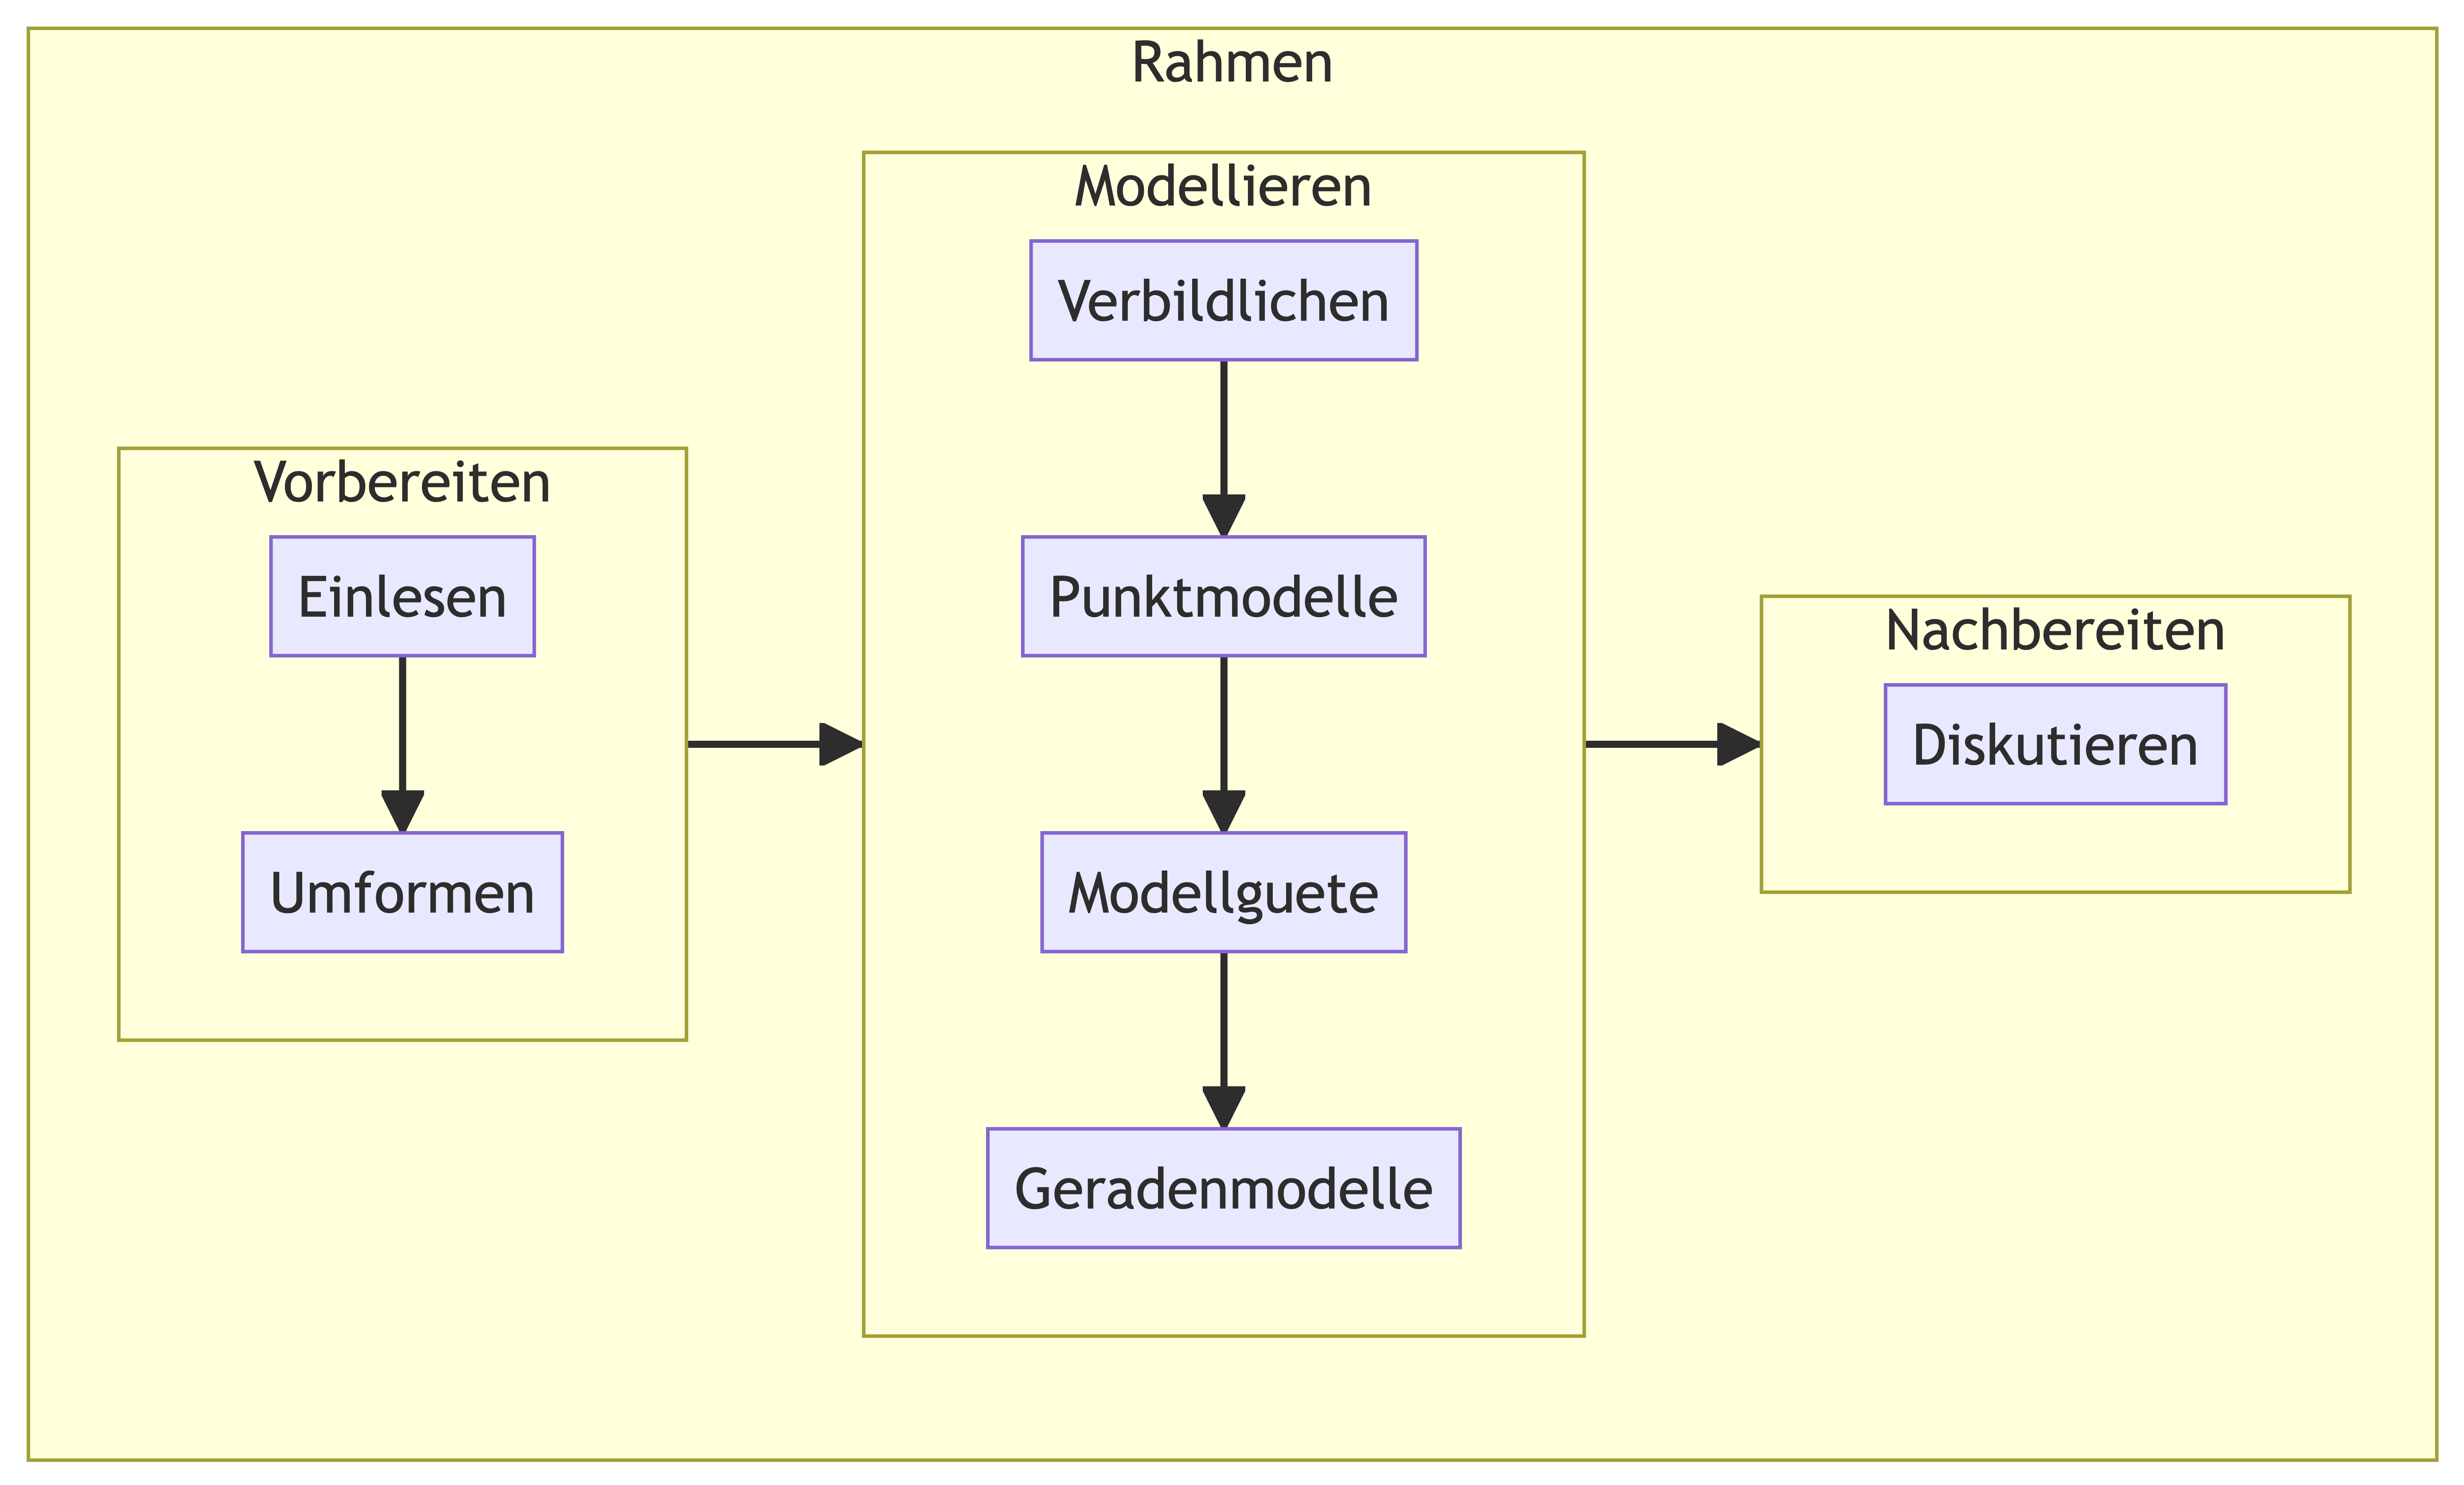
\includegraphics[width=7.93in,height=3.65in]{./index_files/figure-latex/mermaid-figure-1.png}

}

\end{figure}

}

\caption{\label{fig-ueberblick}Überblick über den Inhalt und Verlauf des
Buches}

\end{figure}

\hypertarget{software}{%
\section*{Software}\label{software}}
\addcontentsline{toc}{section}{Software}

\markright{Software}

Installieren Sie
\href{https://data-se.netlify.app/2021/11/30/installation-von-r-und-seiner-freunde/}{R
und seine Freunde}. Für die Bayes-Inferenz brauchen Sie\footnote{nicht
  gleich zu Beginn, aber nach 2-3 Wochen} zusätzliche Software, was
leider etwas Zusatzaufwand erfordert. Lesen Sie
\href{https://data-se.netlify.app/2022/01/28/bayes-software-installieren-f\%C3\%BCr-r/}{hier}
die Hinweise dazu. Installieren Sie die folgende R-Pakete\footnote{falls
  Sie die Pakete schon installiert haben, könnten Sie mal in RStudio auf
  ``update.packages'' klicken}:

\begin{itemize}
\tightlist
\item
  tidyverse
\item
  easystats
\item
  weitere Pakete werden im Unterricht bekannt gegeben (es schadet aber
  nichts, jetzt schon Pakete nach eigenem Ermessen zu installieren)
\end{itemize}

\href{https://github.com/sebastiansauer/Lehre}{R Syntax aus dem
Unterricht} findet sich im Github-Repo bzw. Ordner zum jeweiligen
Semester.

\hypertarget{pdf-version}{%
\section*{PDF-Version}\label{pdf-version}}
\addcontentsline{toc}{section}{PDF-Version}

\markright{PDF-Version}

-- EXPERIMENTAL 🔬🧪 -- EXPERIMENTAL

Von diesem ``Webbuch'' (HTML-Format) gibt es
\href{_book/statistik1.pdf}{hier eine PDF-Version}. Die PDF-Version
eignet sich zum Ausdrucken und zur Offline-Nutzung.

Allerdings wurden die Inhalte \emph{in erster Linie für ein
Webbuch-Format} formatiert, die PDF-Ausgabe ist daher nicht ideal. Es
ist empfehlenswert, mit der Webbuch-Version zu arbeiten. Außerdem wird
die PDF-Version nicht ganz aktuell gehalten - die aktuelle Version ist
immer die Webbuch-Variante. Prüfen Sie im Zweifel das Datum der
Erstellung des Dokuments.

\hypertarget{lernhilfen}{%
\section*{Lernhilfen}\label{lernhilfen}}
\addcontentsline{toc}{section}{Lernhilfen}

\markright{Lernhilfen}

\hypertarget{videos}{%
\subsection*{Videos}\label{videos}}
\addcontentsline{toc}{subsection}{Videos}

Auf dem
\href{https://www.youtube.com/channel/UCkvdtj8maE7g-SOCh4aDB9g}{YouTube-Kanal
des Autors} finden sich eine Reihe von Videos mit Bezug zum Inhalt
dieses Buchs. Besonders
\href{https://youtube.com/playlist?list=PLRR4REmBgpIEzVFLvzCn76TB2VS4jXcfg}{diese
Playlist} passt zu den Inhalten dieses Buchs.

\hypertarget{online-zusammenarbeit}{%
\subsection*{Online-Zusammenarbeit}\label{online-zusammenarbeit}}
\addcontentsline{toc}{subsection}{Online-Zusammenarbeit}

Hier finden Sie einige Werkzeuge, die das Online-Zusammenarbeiten
vereinfachen:

\begin{itemize}
\tightlist
\item
  \href{https://frag.jetzt/home}{Frag-Jetzt-Raum zum anonymen Fragen
  stellen während des Unterrichts}. Der Keycode wird Ihnen bei Bedarf
  vom Dozenten bereitgestellt.
\item
  \href{https://de.padlet.com/}{Padlet} zum einfachen (und anonymen)
  Hochladen von Arbeitsergebnissen der Studentis im Unterricht. Wir
  nutzen es als eine Art Pinwand zum Sammeln von Arbeitsbeiträgen. Die
  Zugangsdaten stellt Ihnen der Dozent bereit.
\end{itemize}

\hypertarget{selbstlernkontrolle}{%
\subsection*{Selbstlernkontrolle}\label{selbstlernkontrolle}}
\addcontentsline{toc}{subsection}{Selbstlernkontrolle}

Für jedes Kapitel sind (am Kapitelende) Aufgaben eingestellt, jeweils
mit Lösung. Ein Teil dieser Aufgaben hat eine kurze, eindeutige Lösung
(z.B. ``42'' oder ``Antwort C''); ein (kleiner) Teil der Aufgaben
verlangen komplexere Antworten (z.B. ``Welche Arten von Prioris gibt es
bei \texttt{stan\_glm()}?). Nutzen Sie die Fragen mit eindeutiger,
kurzer Lösung um sich selber zu prüfen. Nutzen Sie die Fragen mit
komplexerer, längerer Lösung, um ein Themengebiet tiefer zu erarbeiten.

\begin{tcolorbox}[enhanced jigsaw, titlerule=0mm, bottomrule=.15mm, opacitybacktitle=0.6, colframe=quarto-callout-note-color-frame, title=\textcolor{quarto-callout-note-color}{\faInfo}\hspace{0.5em}{Hinweis}, coltitle=black, colback=white, arc=.35mm, breakable, toptitle=1mm, opacityback=0, bottomtitle=1mm, left=2mm, leftrule=.75mm, rightrule=.15mm, toprule=.15mm, colbacktitle=quarto-callout-note-color!10!white]

Fortwährendes Feedback zu Ihrem Lernfortschritt ist wichtig, damit Sie
Ihre Lernbemühungen steuern können. Bearbeiten Sie daher die
bereitgestellten Arbeiten ernsthaft.

\end{tcolorbox}

\hypertarget{forum}{%
\subsection*{Forum}\label{forum}}
\addcontentsline{toc}{subsection}{Forum}

Nutzen Sie das vom Dozenten bereitgestelle Forum, um Fragen zu stellen
und Fragen zu beantworten.

\hypertarget{modulzeitplan}{%
\section*{Modulzeitplan}\label{modulzeitplan}}
\addcontentsline{toc}{section}{Modulzeitplan}

\markright{Modulzeitplan}

\begin{longtable}{rlrl}
\toprule
Nr & Thema & Datum & Kommentar \\ 
\midrule
1 & Fragen stellen & 13.3. - 19.3. & Lehrbeginn ist am Mi., 15.3.23 \\ 
2 & Daten aufbereiten & 20.3. - 26.3. & NA \\ 
3 & Daten aufbereiten & 27.3. - 2.4. & NA \\ 
4 & Daten verbildlichen & 3.4. - 9.4 & Karwoche (kein Unterricht am Do. und Fr.) \\ 
5 & Daten verbildlichen & 10.4. - 16.4. & Osterwoche (kein Unterricht am Mo. und Di.) \\ 
6 & Punktmodelle & 17.4. - 23.4. & NA \\ 
7 & Punktmodelle & 24.4. - 30.4. & NA \\ 
8 & Ungewissheit quantifizieren & 1.5. - 7.5. & Maifeiertag (kein Unterricht am Mo.) \\ 
9 & Ungewissheit quantifizieren & 8.5. - 14.5. & NA \\ 
10 & Fallstudien & 15.5. - 21.5. & NA \\ 
11 & - & 22.5. - 28.5. & Blockwocke - kein regulärer Unterricht \\ 
12 & Geradenmodell & 29.6. - 4.6. & Pfingstwoche (kein Unterricht am Mo. und Di.) \\ 
13 & Geradenmodell & 5.6. - 11.6. & Fronleichnam (kein Unterricht am Do. und Fr.) \\ 
14 & Antworten diskutieren & 12.6. - 18.6. & NA \\ 
15 & Fallstudien & 19.6. - 25.6. & NA \\ 
16 & Abschluss & 26.6. - 2.7. & Letzter Lehrtag ist Fr., 30.6. \\ 
\bottomrule
\end{longtable}

\hypertarget{literatur}{%
\section*{Literatur}\label{literatur}}
\addcontentsline{toc}{section}{Literatur}

\markright{Literatur}

Pro Thema wird Literatur ausgewiesen.

\hypertarget{organisatorische-hinweise}{%
\section*{Organisatorische Hinweise}\label{organisatorische-hinweise}}
\addcontentsline{toc}{section}{Organisatorische Hinweise}

\markright{Organisatorische Hinweise}

\hypertarget{sicherheitsunterweisung}{%
\section*{Sicherheitsunterweisung}\label{sicherheitsunterweisung}}
\addcontentsline{toc}{section}{Sicherheitsunterweisung}

\markright{Sicherheitsunterweisung}

\begin{itemize}
\tightlist
\item
  Der Dozent weist auf Fluchtwege und auf die Sammelstelle hin (abhängig
  vom Seminarraum).
\item
  Flucht- und Rettungspläne hängen im Gebäude aus; bitte betrachten Sie
  sie sorgfältig. Prägen Sie sich die Rettungswege, den Ort der
  Sammelstelle sowie von Feuerlöschern und Brandmeldeeinrichtungen gut
  ein.
\item
  Bei Alarm: Ruhe bewahren. Der Dozent weist an, den Raum sofort zu
  verlassen und geordnet über den kürzesten Weg zur Sammelstelle zu
  gehen. Tun Sie das.
\item
  Prüfen Sie, ob niemand zurückgelassen ist (z. B. auf der Toilette).
\item
  Fluchtwege (z. B. Fluren und Treppen) dürfen nicht versperrt sein.
\item
  Notausgänge müssen ausgeschildert und frei zugänglich sein.
\item
  Aufzüge dürfen im Brandfall nicht verwendet werden. Lebensgefahr!
\item
  Im Brandfall sind Fenster und Türen zu schließen (aber nicht zu
  verriegeln!).
\item
  Hilflose Personen sind mitzunehmen.
\item
  Brände sind zu bekämpfen, aber die sichere Evakuierung hat Vorrang.
\item
  Bei Bränden ist sofort die Feuerwehr zu alarmieren.
\item
  Bei einem Hupton ist das Gebäude sofort zu verlassen und die
  Sammelstelle aufzusuchen. Brandschutztüren sind stets geschlossen zu
  halten.
\item
  Prägen Sie sich die Position von Feuerlöschern und
  Erste-Hilfe-Material gut ein.
\end{itemize}

\hypertarget{organisatorisches}{%
\section*{Organisatorisches}\label{organisatorisches}}
\addcontentsline{toc}{section}{Organisatorisches}

\markright{Organisatorisches}

\begin{itemize}
\tightlist
\item
  Bitte laden Sie sich rechtzeitig die Materialien herunter.
\item
  Beachten Sie die Vorbereitungshinweise zur ersten Unterrichtsstunde
  und für die einzelnen Termine.
\item
  Ein Foliensatz kann kein Lehrbuch ersetzen; falls Sie bei einem Termin
  gefehlt haben oder Ihre Aufzeichnung lückenhaft ist, lesen Sie bitte
  in der Literatur nach oder bitten Sie eine/n Kommiliton/in um Hilfe.
\item
  Beachten Sie die Hinweise der Hochschule (s. Moodle) wie die
  Orientierungshilfe, die Klausur- und Studiengangsordnungen. Dort
  finden Sie verbindliche Hinweise zu vielen organisatorischen Fragen.
\item
  Bitte prüfen Sie jetzt schon und in regelmäßigen Abständen die
  Modulseite auf neue Materialien.
\item
  Nachdem eine Unterrichtseinheit abgeschlossen ist, ändert der Dozent
  grundsätzlich nichts mehr an den Materialien (in Ausnahmefällen wie
  etwa der Korrektur eines Fehler informiert der Dozent schriftlich).
\item
  Es können sich Aktualisierungen des Unterrichtsmaterials ergeben.
  Bitte prüfen Sie regelmäßig, ob neues Material eingestellt ist.
  Nachdem der Unterricht stattgefunden hat, wird das Material aber nicht
  mehr geändert, so dass Sie Sicherheit für das Lernen haben.
\end{itemize}

\hypertarget{pruxe4senzunterricht}{%
\section*{Präsenzunterricht}\label{pruxe4senzunterricht}}
\addcontentsline{toc}{section}{Präsenzunterricht}

\markright{Präsenzunterricht}

\begin{itemize}
\tightlist
\item
  Beachten Sie aktuell geltenden Hygienevorschriften.
\item
  Bitte meiden Sie datenhungrige Applikationen wie das Streamen von
  Filmen -- Sie behindern den Unterricht und verärgern damit andere
  Studierende (in diesem oder anderen Kursen).
\item
  Bitte bringen Sie einen Computer (mit Internetanschluss) in alle
  Präsenztermine mit. Bringen Sie ggf. Ersatzbatterien und/oder
  Verlängerungskabel mit - leider sind nicht überall ausreichend
  Steckdosen vorhanden.
\end{itemize}

\hypertarget{rechtliche-hinweise}{%
\section*{Rechtliche Hinweise}\label{rechtliche-hinweise}}
\addcontentsline{toc}{section}{Rechtliche Hinweise}

\markright{Rechtliche Hinweise}

\begin{itemize}
\tightlist
\item
  Dieser Kurs ist lizensiert unter der
  \href{https://github.com/sebastiansauer/bayes-start/blob/main/LICENSE}{MIT
  Lizenz}. Das ist eine permissive Lizenz, die erlaubt, dass Sie diesen
  Kurs frei verwenden können. Sie haben (nur) die Verpflichtung, zu
  zitieren und auf die Lizenzart hinzuweisen.
\item
  Mitarbeit oder Verbesserungsvorschläge: am besten als Github Issue auf
  der Github-Seite dieses Projekts einstellen.
\item
  Für die Inhalte von Links kann keine Haftung übernommen werden.
\item
  Aus Datenschutzgründen dürfen Teilnehmis den Unterricht (Video, Ton,
  sonstige) nicht aufnehmen.
\end{itemize}

\hypertarget{datenschutz}{%
\section*{Datenschutz}\label{datenschutz}}
\addcontentsline{toc}{section}{Datenschutz}

\markright{Datenschutz}

\begin{itemize}
\tightlist
\item
  Einige Teile des Unterrichts werden u.U. aufgenommen.
\item
  Die Aufnahme erfolgt nur nach vorheriger Information durch den
  Dozenten.
\item
  Bei den Bild-Aufnahmen wird nur der Bildschirm des Dozenten
  aufgenommen; außerdem wird der Ton aufgenommen.
\item
  Bitte verzichten Sie daher während der Aufnahme auf Zoom-Reaktionen
  wie Hand heben, da diese u.U. mit Ihrem Namen auf dem Bildschirm des
  Dozenten und damit auf der Aufnahme zu sehen sind.
\item
  Während einer Aufnahme dürfen aus Datenschutzgründen keine
  Wortbeiträge zu hören sein, die Personen identifizieren.
\item
  Bitte verzichten Sie während der Aufnahme daher auf Wortbeiträge. -
  Der Dozent informiert umgehend, wenn er die Aufnahme beendet.
\item
  Die Aufnahmen werden im Internet (z.B. YouTube) frei veröffentlicht.
  Solche offenen Beiträge im Internet können u.U. in Zukunft nicht
  kontrolliert werden, insbesondere können sie unkontrolliert verbreitet
  und kommentiert werden.
\item
  Der Dozent hat u.U. keinen Einfluss auf Verbreitung, Kommentare oder
  sonstige Weiterverwendung.
\item
  Alle Rechte an den Aufnahmen liegen beim Dozenten.
\item
  Aufnahmen des Unterrichts durch die Studentis sind nicht erlaubt.
\end{itemize}

\hypertarget{it}{%
\section*{IT}\label{it}}
\addcontentsline{toc}{section}{IT}

\markright{IT}

\begin{itemize}
\tightlist
\item
  Sie benötigen einen Computer für diesen Kurs. Ein Laptop ist ideal
  (ein günstiges Modell ist vollkommen ausreichend); ein Tablett ist
  nicht ideal, reicht aber zur Not, wenn Sie eine Tastatur für das Gerät
  haben.
\item
  \href{https://data-se.netlify.app/2021/11/30/installation-von-r-und-seiner-freunde/}{Bereiten
  Sie bitte R und seine Freunden vor} vor der ersten Unterrichtsstunde.
  Sie können entweder R auf Ihrem Computer installieren oder den
  Cloud-Dienst \emph{RStudio Cloud} nutzen.
\item
  Bitte beachten Sie die Installationshinweise für Software und stellen
  Sie sicher, dass die Software vor Beginn des ersten Termins
  einsatzbereit ist.
\item
  Sorgen Sie dafür, dass Sie in jeder Stunde über eine gute
  Internetverbindung verfügen.
\item
  Bitte stellen Sie sicher, dass Sie Zugriff auf Moodle, Zoom und
  weitere Dienste haben, die wir im Unterricht nutzen (Passwörter dabei
  haben etc.).
\item
  Kontaktieren Sie die IT-Abteilung bei technischen Probleme.
\item
  Für Präsenztermine: Bitte bringen Sie folgende IT-Geräte in jede
  Stunde mit: Laptop mit Stromkabel, Smartphone oder Tablett, Kopfhörer
  inkl. Mikrofon.
\item
  Für Präsenztermine: Ein langer Uni-Tag zehrt an der Batterie; nicht
  nur an Ihrer, sondern auch in Ihrem Laptop und Smartphone. Ggf. kann
  eine Zusatzbatterie (Akku-Pack) hilfreich sein. Bei schlechter
  WLAN-Verbindung kann ein Hotspot über das Handy eine Lösung sein.
\item
  Bitte lesen Sie auch die Hinweise zur Software, die wir in diesem
  Modul benötigen.
\item
  Stellen Sie sicher, dass Sie die jeweils aktuelle Version für die in
  diesem Kurs verwendete Software verwenden (z.B. bei Zoom gibt es viele
  Aktualisierungen).
\item
  Updaten Sie ggf. R, RStudio und Ihre R-Pakete.
\end{itemize}

\hypertarget{ich-brauche-hilfe.-was-soll-ich-tun}{%
\section*{Ich brauche Hilfe. Was soll ich
tun?}\label{ich-brauche-hilfe.-was-soll-ich-tun}}
\addcontentsline{toc}{section}{Ich brauche Hilfe. Was soll ich tun?}

\markright{Ich brauche Hilfe. Was soll ich tun?}

\begin{itemize}
\tightlist
\item
  Versuchen Sie erst selber, das Problem zu lösen. Manchmal hilft etwas
  Abstand (Pause, drüber schlafen), um ein Problem klarer zu sehen (oder
  es als nicht mehr so wichtig zu sehen).
\item
  Fragen Sie Kommilitonis.
\item
  Recherchen Sie (online) nach einer Lösung.
\item
  Posten Sie das Problem im Forum oder einem Online-Forum. Wichtig:
  Stellen Sie Ihrem Post ein
  \href{https://data-se.netlify.app/2022/01/31/erbie-einfache-reproduzierbare-beispiele-ihres-problems-mit-r-syntax/}{Erbie}
  bei.
\item
  Besuchen Sie die Sprechstunde des Dozenten.
\item
  Schreiben Sie möglichst keine Email, sondern posten Sie Ihre Frage im
  Forum o.Ä., da die meisten Fragen für Ihre Kommilitonis auch nützlich
  sein können (eine Ausnahme sind natürlich individuelle, persönliche
  Angelegenheiten, die nicht den Stoff betreffen).
\end{itemize}

\hypertarget{videokonferenzen}{%
\section*{Videokonferenzen}\label{videokonferenzen}}
\addcontentsline{toc}{section}{Videokonferenzen}

\markright{Videokonferenzen}

\begin{itemize}
\tightlist
\item
  Ihr Dozent informiert Sie, ob Videokonferenzen in diesem Modul
  angeboten werden.
\item
  Für Videokonferenzen/Webinare in diesem Modul wird die Software Zoom
  verwendet. Zur Einwahl benötigen Sie eine Zoom-Meeting-ID bzw. die
  dazu gehörige URL (Link); außerdem benötigen Sie ggf. ein zugehöriges
  Passwort. Diese Informationen werden Ihnen vom Dozenten zugestellt-.
\item
  Für die Teilnahme an der Videokonferenz können Sie einen
  internetfähigen Rechner oder Tablet/Smartphone verwenden. Alternativ
  können Sie den Zoom-Client auf Ihrem Computer installieren (die
  Installation auf dem Rechner ist zu empfehlen).
\item
  Ein paar Minuten vor Unterrichtsbeginn da sein, hilft beim Ankommen
  und um etwaige technische Probleme auszuräumen.
\item
  -Wenn jede(r) Hintergrundgeräusche vermeidet (auch die Tastatur kann
  ziemlich laute Geräusche verursachen), verstehen wir uns alle gut.
\item
  Das Mikro auszuschalten, wenn man gerade nichts sagen möchte, gibt
  Freiheit, doch nicht ganz leise zu sein, ohne die anderen zu stören. -
  Ein Headset ist hilfreich, um Rückkopplungsgeräusche (Echo) zu
  vermeiden.
\item
  Eine einigermaßen schnelle Internetverbindung ist nötig.
\item
  Ich empfehle, eine Webcam anzuschließen (bzw. freigeben), so dass wir
  uns sehen können. Das ist der Qualität des Unterrichts zuträglich.
\item
  Hilfe zu Zoom findet sich hier: https://support.zoom.us/hc/de.
\item
  Zu bestimmten Seiten kann der Dienst (Zoom) überlastet sein, so dass
  das Webinar nur eingeschränkt oder nicht möglich ist. In diesem Fall
  erstellt der Dozent ein Video und stellt es im Nachgang über Moodle
  zur Verfügung.
\item
  Die Datenschutzhinweise von Zoom finden Sie
  \href{https://zoom.us/docs/en-us/privacy-and-security.html}{hier.}
\item
  Prüfen Sie regelmäßig, ob Ihr Zoom-Client aktuell ist (sonst updaten).
\item
  Aus Gründen der Sicherheit der Teilnehmis kann der Dozent anonyme
  Teilnahme an Videokonferenzen untersagen.
\item
  Der Chat sollte nur für Themen des Unterrichts verwendet werden (nicht
  für private Themen).
\item
  Aus Sicherheitsgründen kann eine Zoom-Konferenz auf Ihre
  ``offizielle'' E-Mail-Adresse (der Hochschule) begrenzt sein. Mit
  einer anderen, potenziell anonymen E-Mail-Adresse, können Sie also
  u.U. nicht teilnehmen.
\end{itemize}

\hypertarget{streaming}{%
\section*{Streaming}\label{streaming}}
\addcontentsline{toc}{section}{Streaming}

\markright{Streaming}

In einigen Kursen wird Präsenzunterricht plus Streaming angeboten. In
diesem Fall gelten folgende Hinweise:

\begin{itemize}
\tightlist
\item
  Wenn die Teilnehmerzahl am Kurs geringer ist als die Raumkapazität
  (z.B. weniger als 80 Teilnehmis), so haben Sie stets freie Wahl, ob
  Sie in Präsenz beiwohnen oder den Unterricht online verfolgen.
\item
  Übersteigt die Teilnehmerzahl am Kurs die Raumkapazität bis zum
  Doppelten (z.B. 160 Teilnehmis bei 80 Plätzen), so findet der
  Präsenzunterricht zweizügig statt. In der 1. Woche können alle
  Studentis des Zugs A zum Präsenunterricht kommen; in Woche 2 können
  alle Studentis des Zugs B zum Präsenzunterricht kommen. Wer nicht für
  Präsenz eingeteilt ist, kann dem Unterricht online folgen. Auch wer in
  Präsenz eingeteilt ist, kann dem Unterricht jederzeit online folgen.
  Auch wer nicht für Präsenz eingeteilt ist, kann zum Präsenzunterricht
  kommen, FALLS es freie Plätze gibt: Kommen Sie einfach zum Hörsaal,
  wenn es freie Plätze gibt, sind Sie herzlich willkommen (es gilt:
  first come, first serve).
\item
  Sie müssen sich nicht anmelden für Präsenz oder Online.
\item
  Falls die Teilnehmerzahl größer ist als das Doppelte oder es Probleme
  mit dem Prozedere gibt, erfolgt eine neue Planung.
\item
  Ihr Dozent informiert Sie zu den Details, sobald die Teilnehmerzahl
  (grob) feststeht.
\item
  Alle Angaben sind vorbehaltlich neuer Corona-Entwicklungen bzw. der
  Vorgaben der Hochschulleitung dazu.
\end{itemize}

\hypertarget{umgangsformen}{%
\section*{Umgangsformen}\label{umgangsformen}}
\addcontentsline{toc}{section}{Umgangsformen}

\markright{Umgangsformen}

\begin{itemize}
\tightlist
\item
  Freundlicher Umgang miteinander ist selbstverständlich.
\item
  Selbstverständlich sind auch die grundlegenden Formen der höflichen
  Miteinanders (Begrüßung, Ansprache mit Namen, bitte/danke sagen,
  Pünktlichkeit, Verbindlichkeit, \ldots).
\item
  Bei Nichtwissen oder einem inhaltlichen Fehler wird niemand
  bloßgestellt oder lächerlich gemacht.
\item
  Um eine Wortmeldung in einer Videokonferenz anzuzeigen, bietet sich
  die Funktion des Handhebens an.
\item
  In Breakout-Sessions (in Zoom) sollte aktiv mitgearbeitet werden, wer
  das nicht möchte, betritt den Breakout-Room nicht.
\item
  Spricht man eine Person in einer Videokonferenz an, sollte die Kamera
  angeschaltet sein.
\end{itemize}

\hypertarget{wenn-der-unterricht-ausfuxe4llt}{%
\section*{Wenn der Unterricht
ausfällt}\label{wenn-der-unterricht-ausfuxe4llt}}
\addcontentsline{toc}{section}{Wenn der Unterricht ausfällt}

\markright{Wenn der Unterricht ausfällt}

\begin{itemize}
\tightlist
\item
  Im Krankheitsfall werden Sie möglichst frühzeitig informiert (via
  Moodle); das kann bedeuten, dass Sie am Morgen eine Nachricht
  bekommen, dass der Unterricht des jeweiligen Tages ausfällt.
\item
  Leider muss der Unterricht in einigen Fällen aufgrund anderer
  Dienstverpflichtungen des Dozenten entfallen; ein Beispiel sind
  Berungskomissionen (Auswahlgespräche für neu einzustellende
  Professor:innen).
\item
  Aufgrund gesetzlicher Feiertage sowie hochschulweit geltenden
  lehrfreien Tagen fallen jedes Semester einige Tage für den Unterricht
  aus. Bitte informieren Sie sich auf der zentralen Hochschulseite dazu.
\item
  Falls der Unterricht ausfällt, heißt das \emph{nicht}, dass der für
  die jeweilige Woche geplante Stoff obsolet ist. Viel mehr ist Ihre
  Pflicht, den Stoff selbständig zu erarbeiten. Natürlich können Sie bei
  Fragen jederzeit Ihren Dozenten kontaktieren.
\end{itemize}

\hypertarget{salvatorische-klausel}{%
\section*{Salvatorische Klausel}\label{salvatorische-klausel}}
\addcontentsline{toc}{section}{Salvatorische Klausel}

\markright{Salvatorische Klausel}

\begin{itemize}
\tightlist
\item
  Diese Hinweise hier gelten nur insofern Ihre Dozentis Ihnen nicht
  andere Hinweise geben :-)
\end{itemize}

\hypertarget{technische-details}{%
\section*{Technische Details}\label{technische-details}}
\addcontentsline{toc}{section}{Technische Details}

\markright{Technische Details}

Dieses Dokument wurde erzeugt am/um 2023-02-02 08:35:52.

\begin{verbatim}
## - Session info ---------------------------------------------------------------
##  setting  value
##  version  R version 4.2.1 (2022-06-23)
##  os       macOS Big Sur ... 10.16
##  system   x86_64, darwin17.0
##  ui       X11
##  language (EN)
##  collate  en_US.UTF-8
##  ctype    en_US.UTF-8
##  tz       Europe/Berlin
##  date     2023-02-02
##  pandoc   2.19.2 @ /Applications/RStudio.app/Contents/Resources/app/quarto/bin/tools/ (via rmarkdown)
## 
## - Packages -------------------------------------------------------------------
##  package     * version date (UTC) lib source
##  assertthat    0.2.1   2019-03-21 [1] CRAN (R 4.2.0)
##  cellranger    1.1.0   2016-07-27 [1] CRAN (R 4.2.0)
##  cli           3.6.0   2023-01-09 [1] CRAN (R 4.2.0)
##  codetools     0.2-18  2020-11-04 [2] CRAN (R 4.2.1)
##  colorout    * 1.2-2   2022-06-13 [1] local
##  colorspace    2.0-3   2022-02-21 [1] CRAN (R 4.2.0)
##  DBI           1.1.3   2022-06-18 [1] CRAN (R 4.2.0)
##  digest        0.6.31  2022-12-11 [1] CRAN (R 4.2.0)
##  dplyr         1.0.10  2022-09-01 [1] CRAN (R 4.2.0)
##  evaluate      0.19    2022-12-13 [1] CRAN (R 4.2.0)
##  fansi         1.0.3   2022-03-24 [1] CRAN (R 4.2.0)
##  fastmap       1.1.0   2021-01-25 [1] CRAN (R 4.2.0)
##  generics      0.1.3   2022-07-05 [1] CRAN (R 4.2.0)
##  ggplot2       3.4.0   2022-11-04 [1] CRAN (R 4.2.0)
##  glue          1.6.2   2022-02-24 [1] CRAN (R 4.2.0)
##  gt            0.8.0   2022-11-16 [1] CRAN (R 4.2.0)
##  gtable        0.3.1   2022-09-01 [1] CRAN (R 4.2.0)
##  htmltools     0.5.4   2022-12-07 [1] CRAN (R 4.2.0)
##  jsonlite      1.8.4   2022-12-06 [1] CRAN (R 4.2.0)
##  knitr         1.41    2022-11-18 [1] CRAN (R 4.2.0)
##  lifecycle     1.0.3   2022-10-07 [1] CRAN (R 4.2.0)
##  magrittr      2.0.3   2022-03-30 [1] CRAN (R 4.2.0)
##  munsell       0.5.0   2018-06-12 [1] CRAN (R 4.2.0)
##  pillar        1.8.1   2022-08-19 [1] CRAN (R 4.2.0)
##  pkgconfig     2.0.3   2019-09-22 [1] CRAN (R 4.2.0)
##  R6            2.5.1   2021-08-19 [1] CRAN (R 4.2.0)
##  readxl        1.4.1   2022-08-17 [1] CRAN (R 4.2.0)
##  rlang         1.0.6   2022-09-24 [1] CRAN (R 4.2.0)
##  rmarkdown     2.19    2022-12-15 [1] CRAN (R 4.2.0)
##  rstudioapi    0.14    2022-08-22 [1] CRAN (R 4.2.0)
##  scales        1.2.1   2022-08-20 [1] CRAN (R 4.2.0)
##  sessioninfo   1.2.2   2021-12-06 [1] CRAN (R 4.2.0)
##  stringi       1.7.12  2023-01-11 [1] CRAN (R 4.2.0)
##  stringr       1.5.0   2022-12-02 [1] CRAN (R 4.2.0)
##  tibble        3.1.8   2022-07-22 [1] CRAN (R 4.2.0)
##  tidyselect    1.2.0   2022-10-10 [1] CRAN (R 4.2.0)
##  utf8          1.2.2   2021-07-24 [1] CRAN (R 4.2.0)
##  vctrs         0.5.1   2022-11-16 [1] CRAN (R 4.2.0)
##  withr         2.5.0   2022-03-03 [1] CRAN (R 4.2.0)
##  xfun          0.36    2022-12-21 [1] CRAN (R 4.2.0)
##  yaml          2.3.6   2022-10-18 [1] CRAN (R 4.2.0)
## 
##  [1] /Users/sebastiansaueruser/Rlibs
##  [2] /Library/Frameworks/R.framework/Versions/4.2/Resources/library
## 
## ------------------------------------------------------------------------------
\end{verbatim}

\bookmarksetup{startatroot}

\hypertarget{fragen-stellen}{%
\chapter{Fragen stellen}\label{fragen-stellen}}

\hypertarget{lernsteuerung}{%
\section{Lernsteuerung}\label{lernsteuerung}}

\hypertarget{standort-im-lernpfad}{%
\subsection{Standort im Lernpfad}\label{standort-im-lernpfad}}

Abb. Abbildung~\ref{fig-ueberblick-fragen} zeigt den Standort dieses
Kapitels im Lernpfad und gibt damit einen Überblick über das Thema
dieses Kapitels im Kontext aller Kapitel.

\begin{figure}

{\centering 

\begin{figure}[H]

{\centering 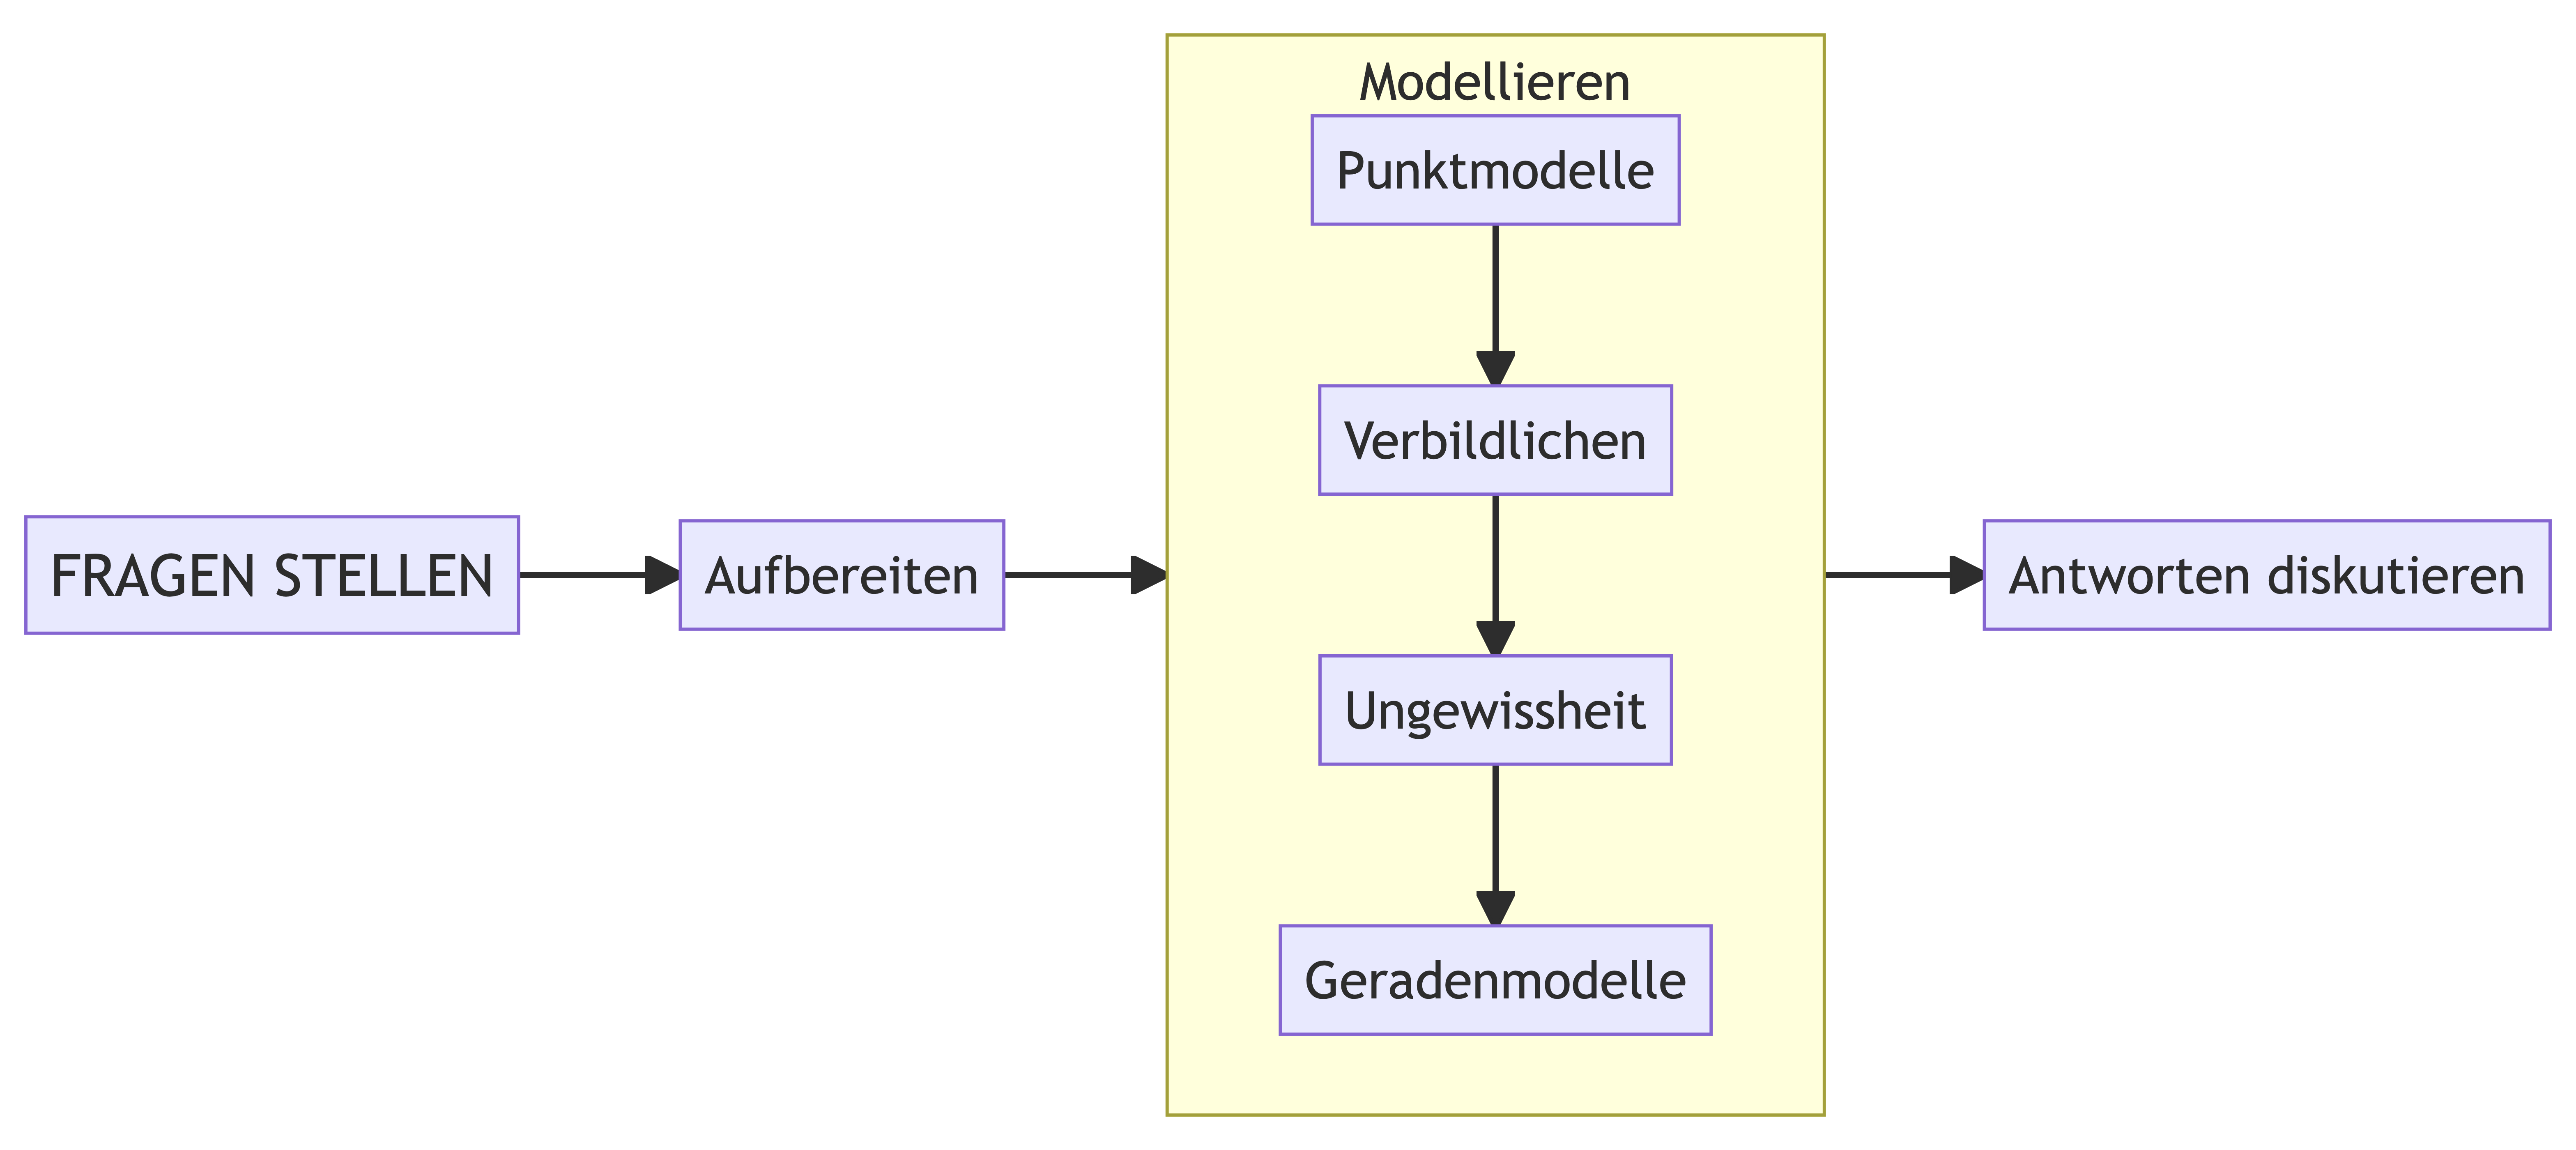
\includegraphics[width=8.3in,height=3.65in]{./fragenstellen_files/figure-latex/mermaid-figure-1.png}

}

\end{figure}

}

\caption{\label{fig-ueberblick-fragen}Überblick über den Inhalt und
Verlauf des Buches}

\end{figure}

\hypertarget{lernziele-1}{%
\subsection{Lernziele}\label{lernziele-1}}

\begin{itemize}
\tightlist
\item
  Sie können eine Definition von Statistik wiedergeben.
\item
  Sie können eine Definition von Daten wiedergeben.
\item
  Sie können den Begriff Tidy-Daten erläutern.
\item
  Sie können Beispiele für verschiedene Skalenniveaus nennen.
\end{itemize}

\hypertarget{was-ist-statistik-und-wozu-ist-sie-gut}{%
\section{Was ist Statistik und wozu ist sie
gut?}\label{was-ist-statistik-und-wozu-ist-sie-gut}}

Es gibt mehrere Definition von Statistik; hier ist eine.

\leavevmode\vadjust pre{\hypertarget{def-statistik}{}}%
\begin{definition}[Statistik]\label{def-statistik}

Statistik fasst Daten zusammen, um wesentliche Informationen den Daten
zu entnehmen und beschreibt die Ungewissheit unserer Schlüsse Kaplan
(2009), Poldrack (2023).

\end{definition}

Ein zentrales Vorgehen bei statistischen Analysen ist es, die
\emph{Unterschiedlichkeit der Dinge} zu beschreiben, präziser gesagt:
die \emph{Variation zu quantifizieren}. Betrachten wir dazu das Beispiel
in s. Abbildung~\ref{fig-groesse}.

\begin{figure}

{\centering 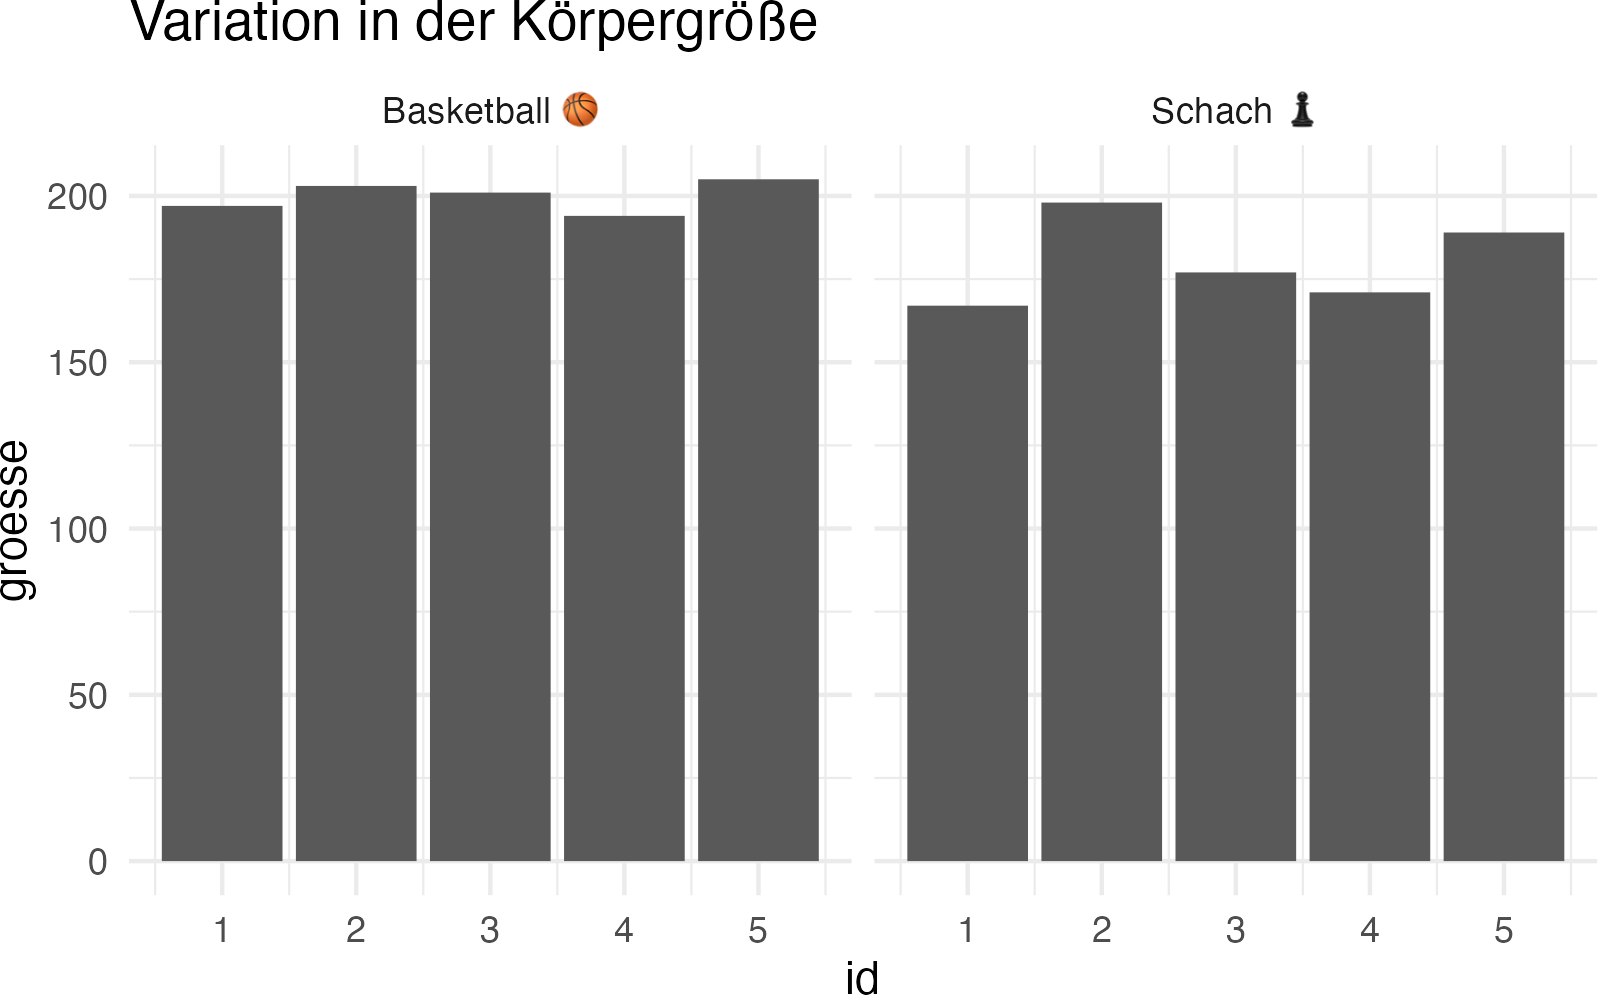
\includegraphics{./fragenstellen_files/figure-pdf/fig-groesse-1.png}

}

\caption{\label{fig-groesse}Wenig Variation in der Körpergröße bei den
Basketballern. Alles lange Kerle. Viel Variation bei den Schachspielern:
Manche sind klein, ander groß.}

\end{figure}

Bei den Basketballern gibt es \emph{wenig} Variation in der Körpergröße
- alle sind groß, ähnlich groß. Bei den Schachspielenr gibt es (im
Verhältnis) \emph{viel} Variation: Einige Personen sind groß, andere
klein.

Die Variation (auch ``Variabilität'' genannt) kann man auch gut so
darstellen wie in s. Abbildung~\ref{fig-variab} gezeigt.

\begin{figure}

{\centering 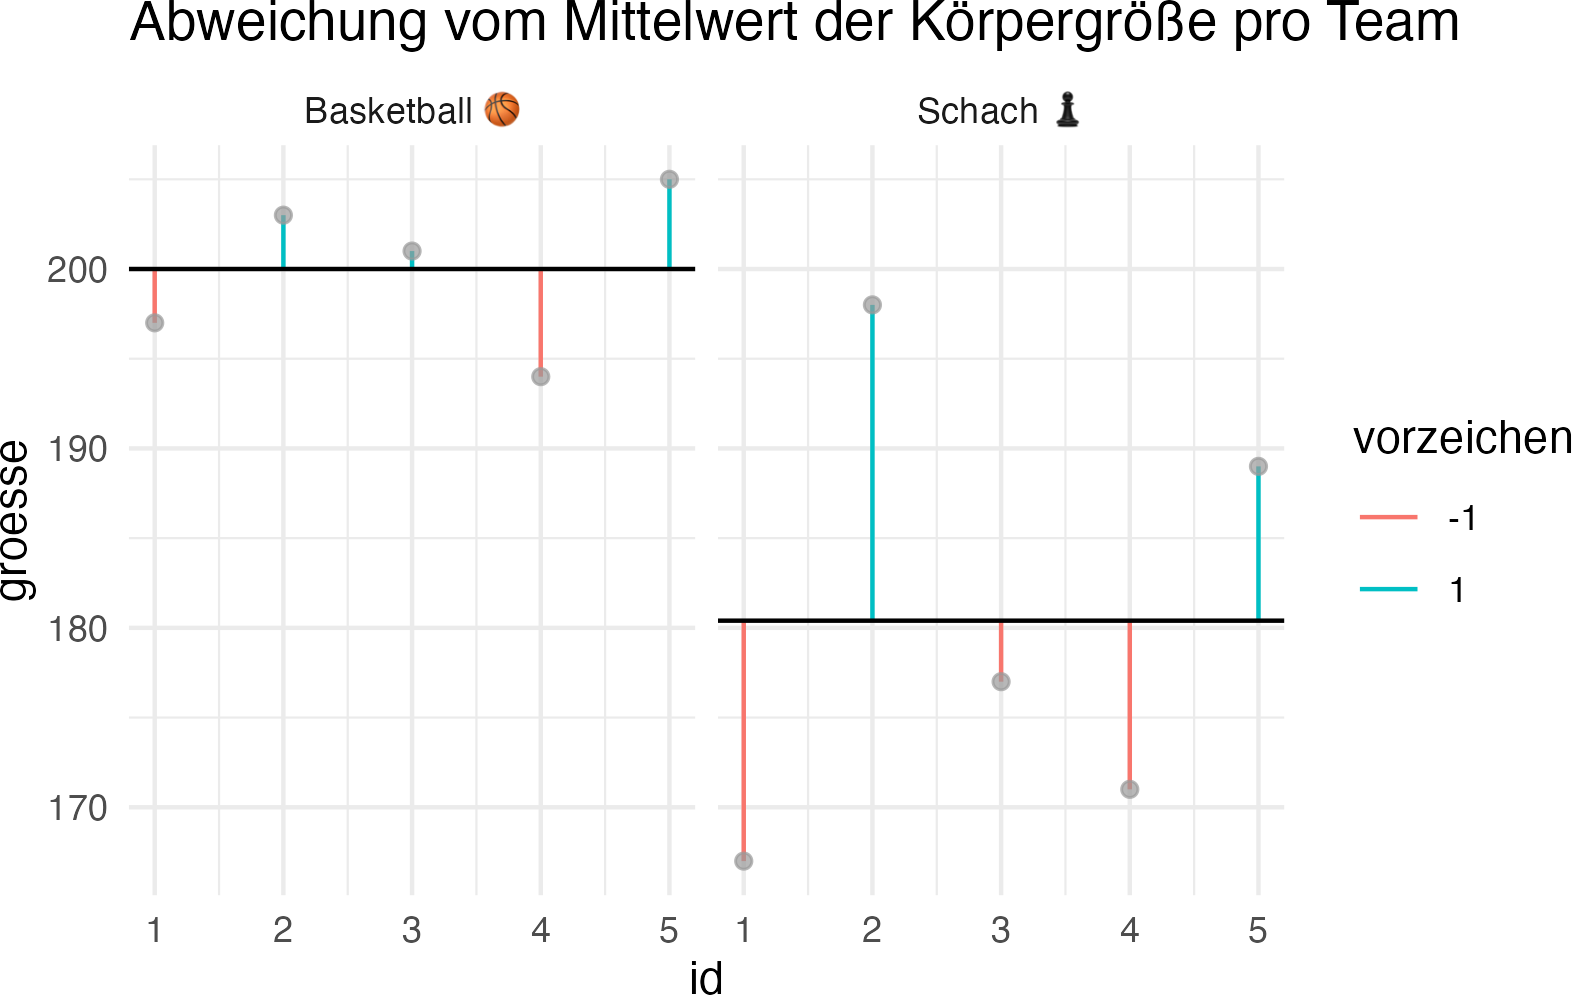
\includegraphics{./fragenstellen_files/figure-pdf/fig-variab-1.png}

}

\caption{\label{fig-variab}Die Abweichungen der einzelnen Personen von
der mittleren Körpergröße ihres Teams}

\end{figure}

Eine \emph{Abweichung} (auch \emph{Residium}) genannt, zeigt die
Differenz von Mittelwert und dem Wert der Körpergröße bei der jeweiligen
Person. Wenn wir allgemein von einer Person \(i\) sprechen, die
Körpergröße mit \(x\) bezeichnen und den Mittelwert der Körpergröße als
\(\bar{x}\) (``x quer''), dann können wir knapp und präzise das Residuum
\(r\) so definieren: \(r = x_i - \bar{x}\)

\hypertarget{was-ist-das-ziel-ihrer-analyse}{%
\section{Was ist das Ziel Ihrer
Analyse?}\label{was-ist-das-ziel-ihrer-analyse}}

\hypertarget{arten-von-zielen}{%
\subsection{Arten von Zielen}\label{arten-von-zielen}}

\begin{figure}

{\centering 

\begin{figure}[H]

{\centering 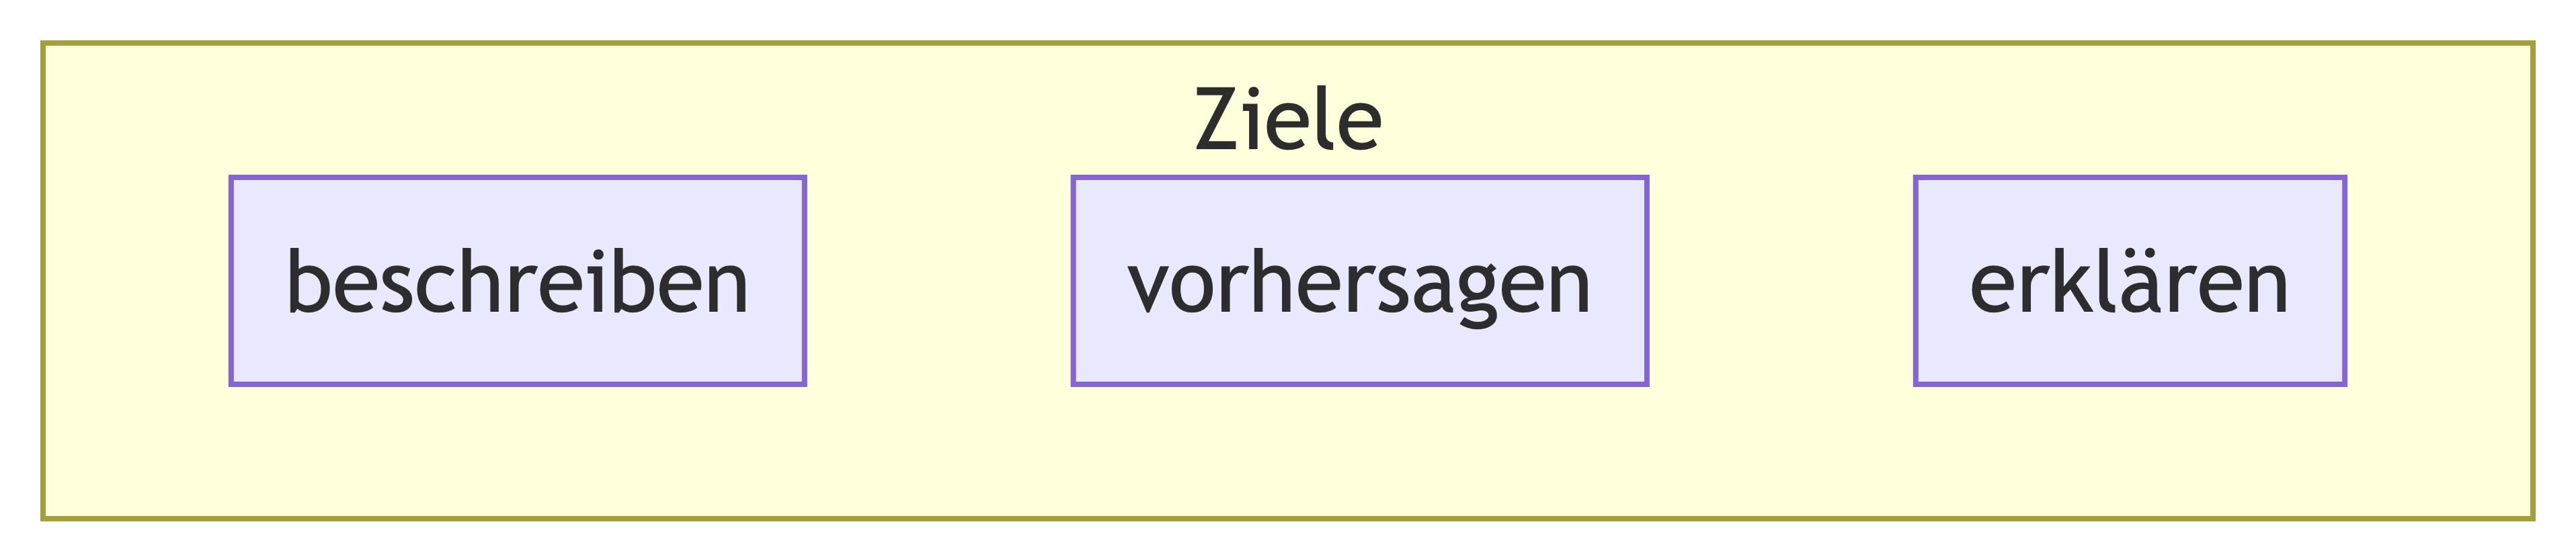
\includegraphics[width=4.99in,height=1.09in]{./fragenstellen_files/figure-latex/mermaid-figure-5.png}

}

\end{figure}

}

\caption{\label{fig-ziele}Zielarten einer Datenanalyse}

\end{figure}

Beispiele für die einzelnen Zielarten der Datenanalyse:

\begin{itemize}
\tightlist
\item
  \emph{Beschreiben}: ``Wie groß ist der Gender-Paygap in der Branche X
  im Zeitraum Y?''
\item
  \emph{Vorhersagen}: Wenn ich 100 Stunden auf die Statistikklausur
  lernen, welche Note kann ich dann erwarten?
\item
  \emph{Erklären}: Wie viel bringt mir das Lernen auf die
  Statistikklausur?
\end{itemize}

\hypertarget{forschungsfrage}{%
\subsection{Forschungsfrage}\label{forschungsfrage}}

Eine Forschungsfrage ist die Leitfrage Ihrer Analyse. Sie definiert, was
Sie herausfinden wollen. Häufig sind Forschungsfragen so aufgebaut:

\begin{quote}
Hat X einen Einfluss auf Y?
\end{quote}

\leavevmode\vadjust pre{\hypertarget{exm-fofrage1}{}}%
\begin{example}[Forschungsfrage 1]\label{exm-fofrage1}

~

\begin{quote}
Hat Lernen einen Einfluss auf den Prüfungserfolg? Verringert Joggen die
Menge des Hüftgolds? Um welchen Betrag erhöht sich der Umsatz, wenn wir
1000€ mehr Werbung ausgeben?
\end{quote}

\end{example}

\leavevmode\vadjust pre{\hypertarget{exm-fofrage2}{}}%
\begin{example}[Forschungsfrage 2]\label{exm-fofrage2}

Nach dem Studium haben Sie bei einem großen Online-Auktionshaus
angeheuert. Da Sie angaben, sich im Studium \sout{intensiv} etwas mit
Statistik beschäftigt zu haben, hat man Sie in die
F\&E-Abteilung\footnote{Forschung und Entwicklung} gesteckt. Heute ist
es Ihre Aufgabe, Auktionen zur Spielekonsole
\href{https://www.nintendo.de/Wii/Wii-94559.html}{Wii} zu untersuchen,
genauer gesagt, geht es um das Spiel
\href{https://www.nintendo.de/Spiele/Wii/Mario-Kart-Wii-281848.html\#_bersicht}{Mariokart}.
Ihre Forschungsfrage lautet:

\begin{quote}
Welche Produktmerkmale stehen mit einem hohen Verkaufserlös in
Zusammenhang?
\end{quote}

\end{example}

\leavevmode\vadjust pre{\hypertarget{exm-braindrain}{}}%
\begin{example}[Aus der Forschung:
Smartphone-Brain-Drain]\label{exm-braindrain}

Ward u.~a. (2017) untersuchten die Forschungsfrage, ob die bloße
Gegenwart eines Handies (z.B. wenn es vor Ihnen auf dem Tisch dazu
führt, dass man abgelenkt wird und daher schlechtere kognitive
Leistungen zeigt.

Leider schreiben die Autoren Ihre Hypothese nicht glasklar, aber
implizit ist obige Hypothese herauszulesen:

\begin{quote}
First, smartphones may redirect the orientation of conscious attention
away from the focal task and toward thoughts or behaviors associated
with one's phone. Prior research provides ample evidence that \ldots{}
that this digital distraction adversely affects both performance
\ldots{} and enjoyment.
\end{quote}

Später formulieren Sie Ihre Hypothese noch genauer:

\begin{quote}
In two experiments, we test the hypothesis that the mere presence of
one's own smartphone reduces available cognitive capacity.
\end{quote}

Die Ergebnisse unterstützen Ihre Hypothese, s.
Abbildung~\ref{fig-braindrain}. Im Diagramm ist ersichtlich, dass die
kognitive Leistung (Y-Achse) sowohl in der Kapazität des
Arbeitsgedächtnisses (links) als auch in der fluiden Intelligenz
(rechts) am geringsten ist, wenn das Handy auf dem Schreibtisch (Desk)
liegt. Am besten ist die kognitive Leistung, wenn das Handy nicht im
Raum ist.

\begin{figure}

{\centering 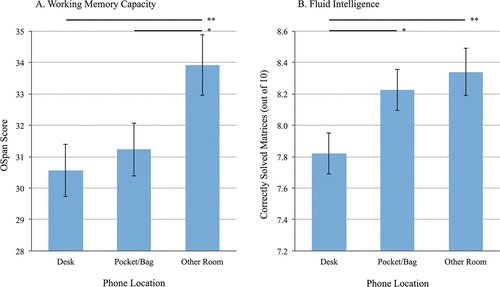
\includegraphics{./img/braindrain1.jpg}

}

\caption{\label{fig-braindrain}Handy in Sichtweite verringert die
kognitiven Ressourcen}

\end{figure}

\end{example}

Eine Forschungsfrage weist häufig folgende Struktur auf, s.
Abbildung~\ref{fig-fo-struktur}.

\begin{figure}

{\centering 

\begin{figure}[H]

{\centering 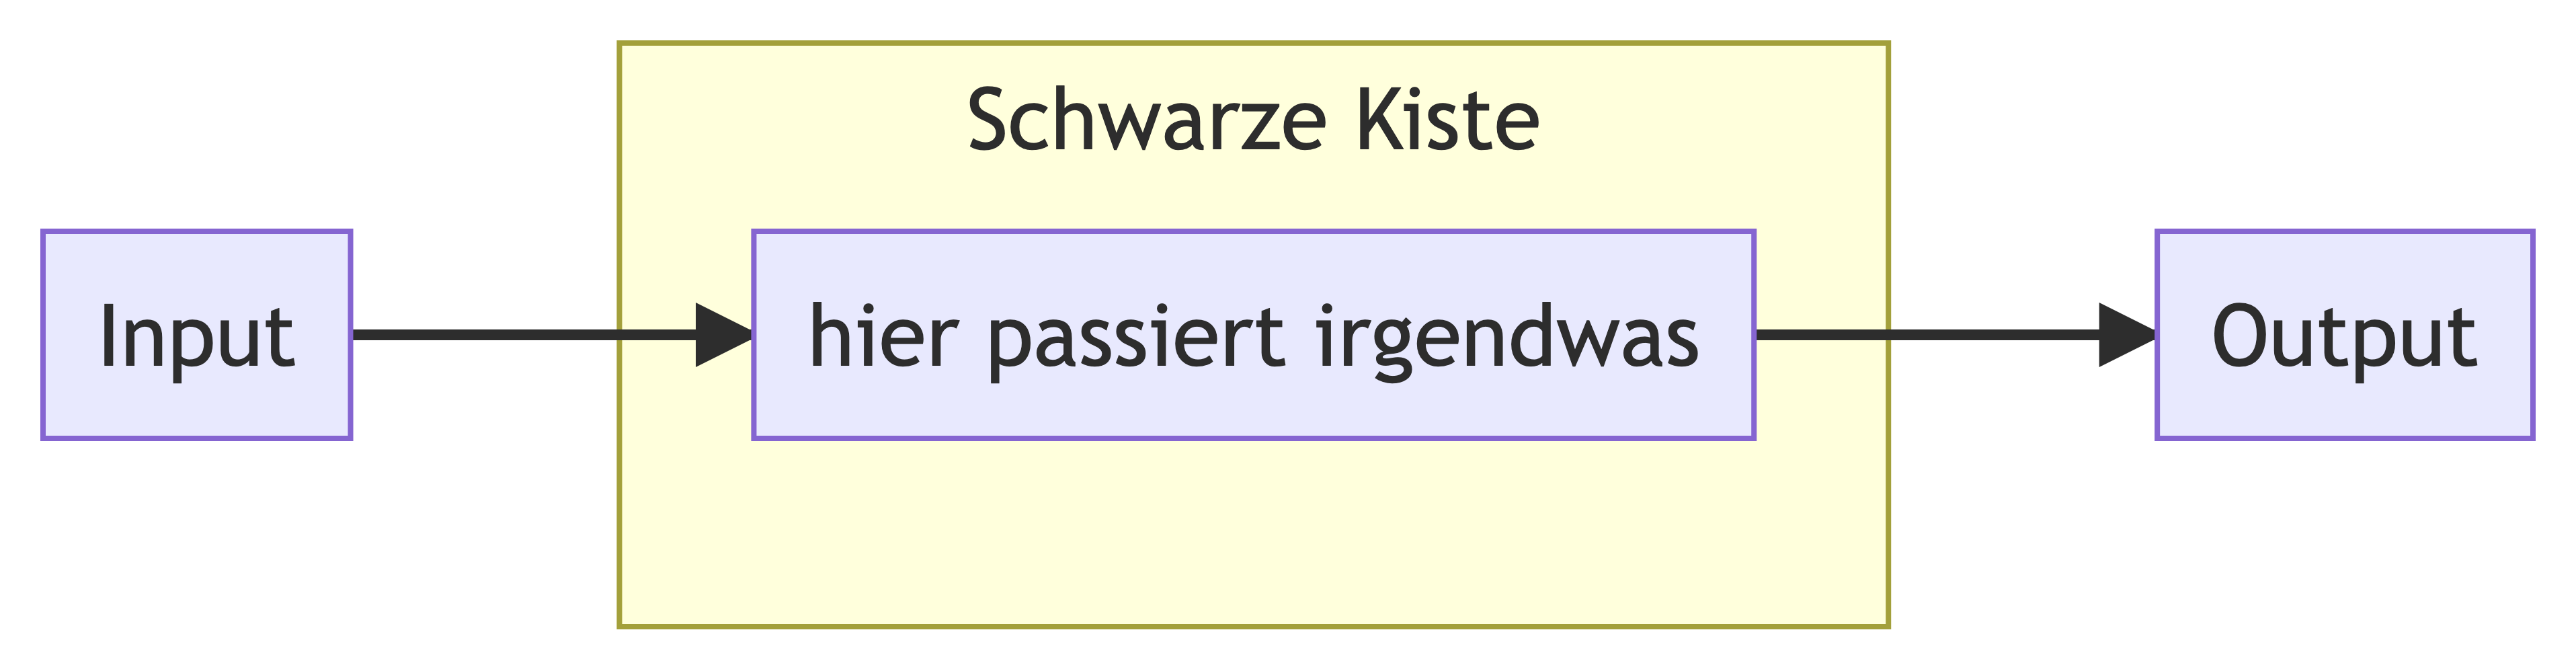
\includegraphics[width=4.99in,height=1.3in]{./fragenstellen_files/figure-latex/mermaid-figure-4.png}

}

\end{figure}

}

\caption{\label{fig-fo-struktur}Struktur eine Forschungsfrage}

\end{figure}

\begin{tcolorbox}[enhanced jigsaw, titlerule=0mm, bottomrule=.15mm, opacitybacktitle=0.6, colframe=quarto-callout-caution-color-frame, title=\textcolor{quarto-callout-caution-color}{\faFire}\hspace{0.5em}{Vorsicht}, coltitle=black, colback=white, arc=.35mm, breakable, toptitle=1mm, opacityback=0, bottomtitle=1mm, left=2mm, leftrule=.75mm, rightrule=.15mm, toprule=.15mm, colbacktitle=quarto-callout-caution-color!10!white]

Es ist ein häufiger Fehler, in der Forschungsfrage zu formulieren ``X
führt zu Y'', aber in der Analyse keine Methode zu verwenden, die
geeignet ist, kausale Zusammenhänge aufzudecken. Es reicht nicht, dass
man z.B. einen (negativen) Zusammenhang zwischen der Häufigkeit von
Smartphone-Nutzung und Konzentrationsfähigkeit findet (Schwaiger und
Tahir 2022), um zu sagen: ``Daddeln macht dumm!''. Es könnte ja z.B.
auch umgekehrt sein. Platt gesagt: ``Dummheit führt zu Daddeln''.
Weitere Erklärungen sind möglich. Vorsicht also mit (vor)schnellen
Aussagen zu kausalen Abhängigkeiten.

\end{tcolorbox}

\hypertarget{was-sind-daten}{%
\section{Was sind Daten?}\label{was-sind-daten}}

\leavevmode\vadjust pre{\hypertarget{def-daten}{}}%
\begin{definition}[Daten]\label{def-daten}

Daten kann man als eine geordnete Folge von Zeichen definieren.

\end{definition}

Daten kommen häufig in Tabellenform vor; so sind sie am besten zu
untersuchen, s. Tabelle~\ref{tbl-daten}.

\hypertarget{tbl-daten}{}
\begin{longtable}[]{@{}rlr@{}}
\caption{\label{tbl-daten}So sehen Daten aus.}\tabularnewline
\toprule()
id & name & note \\
\midrule()
\endfirsthead
\toprule()
id & name & note \\
\midrule()
\endhead
1 & Anna & 1.3 \\
2 & Berta & 2.3 \\
3 & Carla & 3.0 \\
\bottomrule()
\end{longtable}

Die erste Spalte \texttt{id} ist nur eine laufende Nummer. Sie dient
dazu, die einzelnen Beobachtungen (hier Studentis) identifizieren zu
können und birgt ansonsten keine Information. Beispiele für ID-Variabeln
sind z.B. Matrikulationsnummer, Personalausweisnummern oder
Bestellnumern.

\leavevmode\vadjust pre{\hypertarget{exm-daten}{}}%
\begin{example}[Daten zur Forschungsfrage 2]\label{exm-daten}

Hier ist ein Auszug der Daten zur Tabelle \texttt{mariokart}:

\begin{longtable}[]{@{}
  >{\raggedleft\arraybackslash}p{(\columnwidth - 20\tabcolsep) * \real{0.1275}}
  >{\raggedleft\arraybackslash}p{(\columnwidth - 20\tabcolsep) * \real{0.0882}}
  >{\raggedleft\arraybackslash}p{(\columnwidth - 20\tabcolsep) * \real{0.0686}}
  >{\raggedright\arraybackslash}p{(\columnwidth - 20\tabcolsep) * \real{0.0490}}
  >{\raggedleft\arraybackslash}p{(\columnwidth - 20\tabcolsep) * \real{0.0882}}
  >{\raggedleft\arraybackslash}p{(\columnwidth - 20\tabcolsep) * \real{0.0784}}
  >{\raggedleft\arraybackslash}p{(\columnwidth - 20\tabcolsep) * \real{0.0882}}
  >{\raggedright\arraybackslash}p{(\columnwidth - 20\tabcolsep) * \real{0.1078}}
  >{\raggedleft\arraybackslash}p{(\columnwidth - 20\tabcolsep) * \real{0.1176}}
  >{\raggedright\arraybackslash}p{(\columnwidth - 20\tabcolsep) * \real{0.1176}}
  >{\raggedleft\arraybackslash}p{(\columnwidth - 20\tabcolsep) * \real{0.0686}}@{}}
\toprule()
\begin{minipage}[b]{\linewidth}\raggedleft
id
\end{minipage} & \begin{minipage}[b]{\linewidth}\raggedleft
duration
\end{minipage} & \begin{minipage}[b]{\linewidth}\raggedleft
n\_bids
\end{minipage} & \begin{minipage}[b]{\linewidth}\raggedright
cond
\end{minipage} & \begin{minipage}[b]{\linewidth}\raggedleft
start\_pr
\end{minipage} & \begin{minipage}[b]{\linewidth}\raggedleft
ship\_pr
\end{minipage} & \begin{minipage}[b]{\linewidth}\raggedleft
total\_pr
\end{minipage} & \begin{minipage}[b]{\linewidth}\raggedright
ship\_sp
\end{minipage} & \begin{minipage}[b]{\linewidth}\raggedleft
seller\_rate
\end{minipage} & \begin{minipage}[b]{\linewidth}\raggedright
stock\_photo
\end{minipage} & \begin{minipage}[b]{\linewidth}\raggedleft
wheels
\end{minipage} \\
\midrule()
\endhead
150377422259 & 3 & 20 & new & 0.99 & 4.00 & 51.55 & standard & 1580 &
yes & 1 \\
260483376854 & 7 & 13 & used & 0.99 & 3.99 & 37.04 & firstClass & 365 &
yes & 1 \\
320432342985 & 3 & 16 & new & 0.99 & 3.50 & 45.50 & firstClass & 998 &
no & 1 \\
280405224677 & 3 & 18 & new & 0.99 & 0.00 & 44.00 & standard & 7 & yes &
1 \\
170392227765 & 1 & 20 & new & 0.01 & 0.00 & 71.00 & media & 820 & yes &
2 \\
360195157625 & 3 & 19 & new & 0.99 & 4.00 & 45.00 & standard & 270144 &
yes & 0 \\
\bottomrule()
\end{longtable}

Eine Erklärung aller Variablen findet sich
\href{https://www.openintro.org/data/index.php?data=mariokart}{hier}.
Eine Erklärung, was die Namen einer Datentabelle bedeuten, nennt man
\emph{Code Book} or \emph{Data Dictionary}.

\end{example}

\hypertarget{was-ist-eine-variable}{%
\subsection{Was ist eine Variable?}\label{was-ist-eine-variable}}

\leavevmode\vadjust pre{\hypertarget{def-var}{}}%
\begin{definition}[Variable]\label{def-var}

Eine Variable ist ein Platzhalter, der für ein Merkmal steht, das
verschiedene Werte annehmen kann.

\end{definition}

Man kann sich eine Variable wie einen Behälter vorstellen, auf dem mit
einem Stift geschrieben steht, was für eine Art Inhalt darin ist, s.
Abbildung~\ref{fig-var-zuweisen}.

\begin{figure}

{\centering 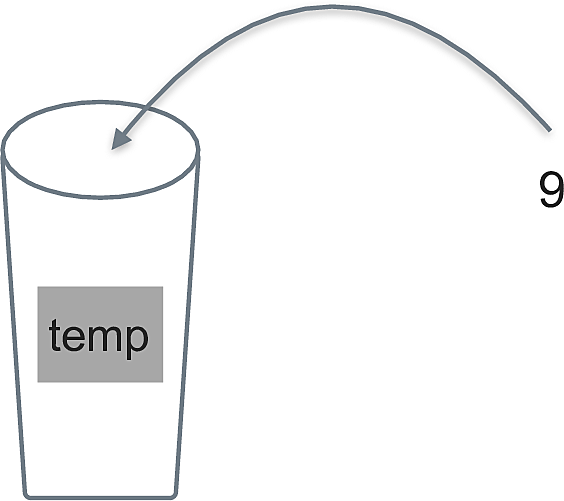
\includegraphics[width=0.25\textwidth,height=\textheight]{./img/Variablen_zuweisen.png}

}

\caption{\label{fig-var-zuweisen}Wir definieren eine Variable ``temp''
mit dem Inhalt ``9''}

\end{figure}

\hypertarget{beobachtungseinheit}{%
\subsection{Beobachtungseinheit}\label{beobachtungseinheit}}

\leavevmode\vadjust pre{\hypertarget{def-beobeinheit}{}}%
\begin{definition}[Beobachtungseinheit]\label{def-beobeinheit}

Beobachtungseinheiten sind die Dinge, die wir untersuchen (beobachten).
Beobachtungseinheiten sind die Träger von Variablen.

\end{definition}

In Tabelle~\ref{tbl-daten} gibt es drei Variablen: \texttt{id},
\texttt{Name} und \texttt{Note}. Es gibt auch drei
Beobachtungseinheiten: \emph{Anna}, \emph{Berta} und \emph{Carla.}

\hypertarget{wert}{%
\subsection{Wert}\label{wert}}

\leavevmode\vadjust pre{\hypertarget{def-wert}{}}%
\begin{definition}[]\label{def-wert}

Ein \emph{Wert} ist der Inhalt einer Variablen.

\end{definition}

In Abbildung~\ref{fig-var-zuweisen} ist der Wert von \texttt{temp} 9.

In Tabelle~\ref{tbl-daten} hat die Variable \texttt{name} drei Elemente:
Anna, Berta, Carla. Der Wert des 2. Elements ist Berta.

Als \emph{Ausprägungen} bezeichnet man die verschiedenen Werte einer
Variablen.

\leavevmode\vadjust pre{\hypertarget{exm-geschlecht}{}}%
\begin{example}[]\label{exm-geschlecht}

In einer Studie wurden zehn Probanden untersucht. Die Variable
\texttt{geschlecht} dokumentiert die Geschlechter der Personen:

\begin{Shaded}
\begin{Highlighting}[]
\NormalTok{geschlecht }\OtherTok{\textless{}{-}} \FunctionTok{c}\NormalTok{(}\StringTok{"Mann"}\NormalTok{, }\StringTok{"Frau"}\NormalTok{, }\StringTok{"Frau"}\NormalTok{, }\StringTok{"Frau"}\NormalTok{, }\StringTok{"Mann"}\NormalTok{,}
                \StringTok{"Frau"}\NormalTok{, }\StringTok{"Mann"}\NormalTok{, }\StringTok{"Mann"}\NormalTok{, }\StringTok{"divers"}\NormalTok{, }\StringTok{"Frau"}\NormalTok{)}
\NormalTok{geschlecht}
\DocumentationTok{\#\#  [1] "Mann"   "Frau"   "Frau"   "Frau"   "Mann"   "Frau"   "Mann"   "Mann"  }
\DocumentationTok{\#\#  [9] "divers" "Frau"}
\end{Highlighting}
\end{Shaded}

In dieser Variable (die aus 10 Werten besteht) finden sich drei
Ausprägungen: divers, Frau, Mann.

\end{example}

\hypertarget{tidy-data}{%
\subsection{Tidy-Data}\label{tidy-data}}

\leavevmode\vadjust pre{\hypertarget{def-tidy}{}}%
\begin{definition}[]\label{def-tidy}

Unter \emph{Tidy-Data} (tidy data) versteht man eine Tabelle, in der
jede Zeile eine Beobachtungseinheit darstellt, jede Spalte eine Variable
und jede Zelle der Tabelle einen Wert, s. Abbildung~\ref{fig-tidy1}.
(Zusätzlich ist noch eine ``Kopfzeile'' erlaubt, in der die Namen der
Variablen stehen.)

\end{definition}

Tabelle~\ref{tbl-daten} ist ein Beispiel für Tidy-Data.

Abbildung~\ref{fig-tidy1} zeigt ein Sinnbild für Tidy-Data (Wickham und
Grolemund 2018).

\begin{figure}

{\centering 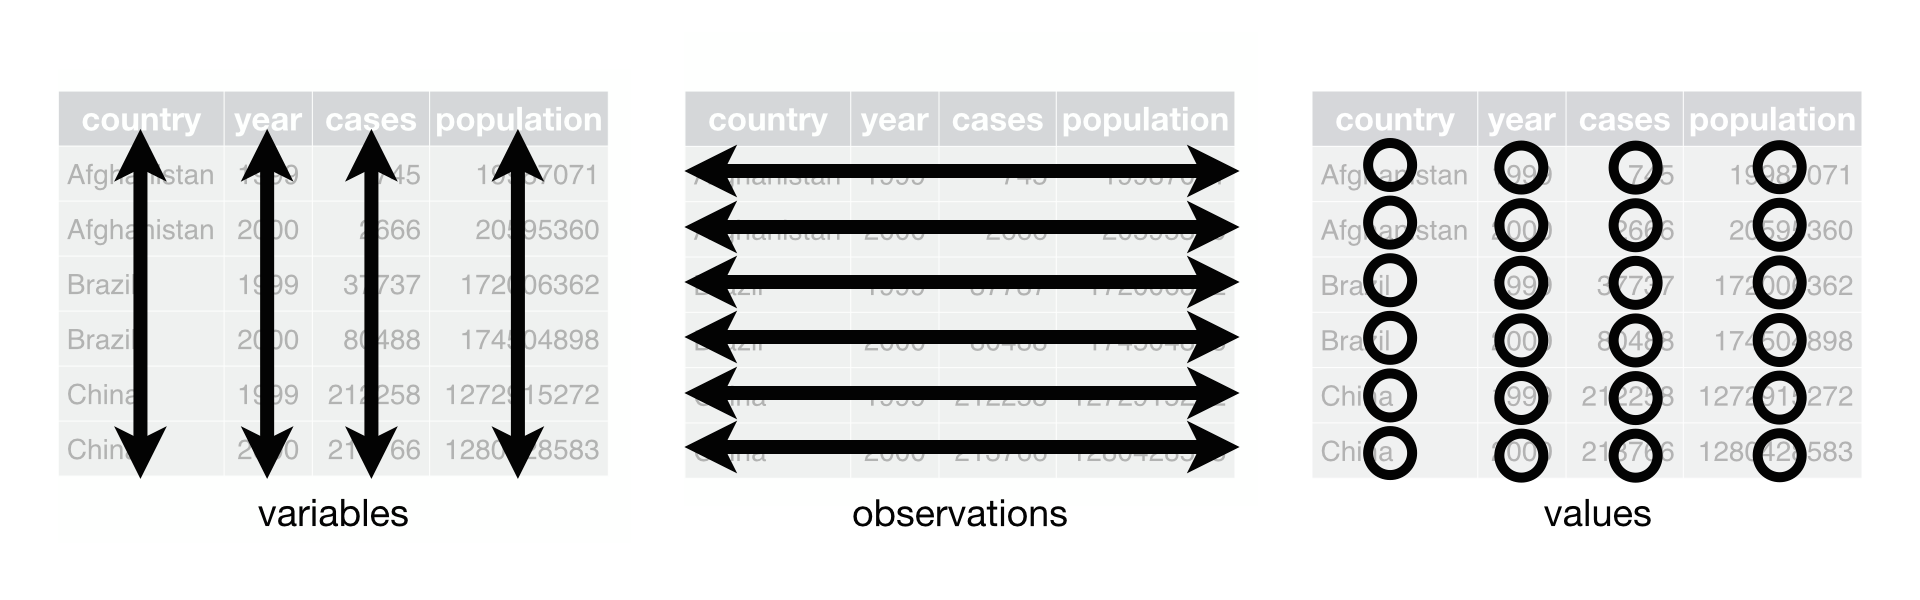
\includegraphics{./img/tidy-1.png}

}

\caption{\label{fig-tidy1}Tidy-Data}

\end{figure}

\begin{tcolorbox}[enhanced jigsaw, titlerule=0mm, bottomrule=.15mm, opacitybacktitle=0.6, colframe=quarto-callout-important-color-frame, title=\textcolor{quarto-callout-important-color}{\faExclamation}\hspace{0.5em}{Wichtig}, coltitle=black, colback=white, arc=.35mm, breakable, toptitle=1mm, opacityback=0, bottomtitle=1mm, left=2mm, leftrule=.75mm, rightrule=.15mm, toprule=.15mm, colbacktitle=quarto-callout-important-color!10!white]

Für eine statistische Analyse ist es fast immer nötig, dass die Daten im
Tidy-Format vorliegen.

\end{tcolorbox}

Der Vorteil des Tidy-Formats ist es, dass man weiß, wie die Daten
aufgebaut sind. Außerdem können Statistikprogramme oft mit dieser Form
am besten umgehen.

Das Tidy-Format wird auch als ``langes'' Format bezeichnet.

Abbildung~\ref{fig-long-wide-anim} zeigt einen Datensatz in der
``langen'' Form, also tidy, und den gleichen Datensatz, umformatiert in
der ``breiten'' Form, nicht-tidy.

\begin{figure}

{\centering 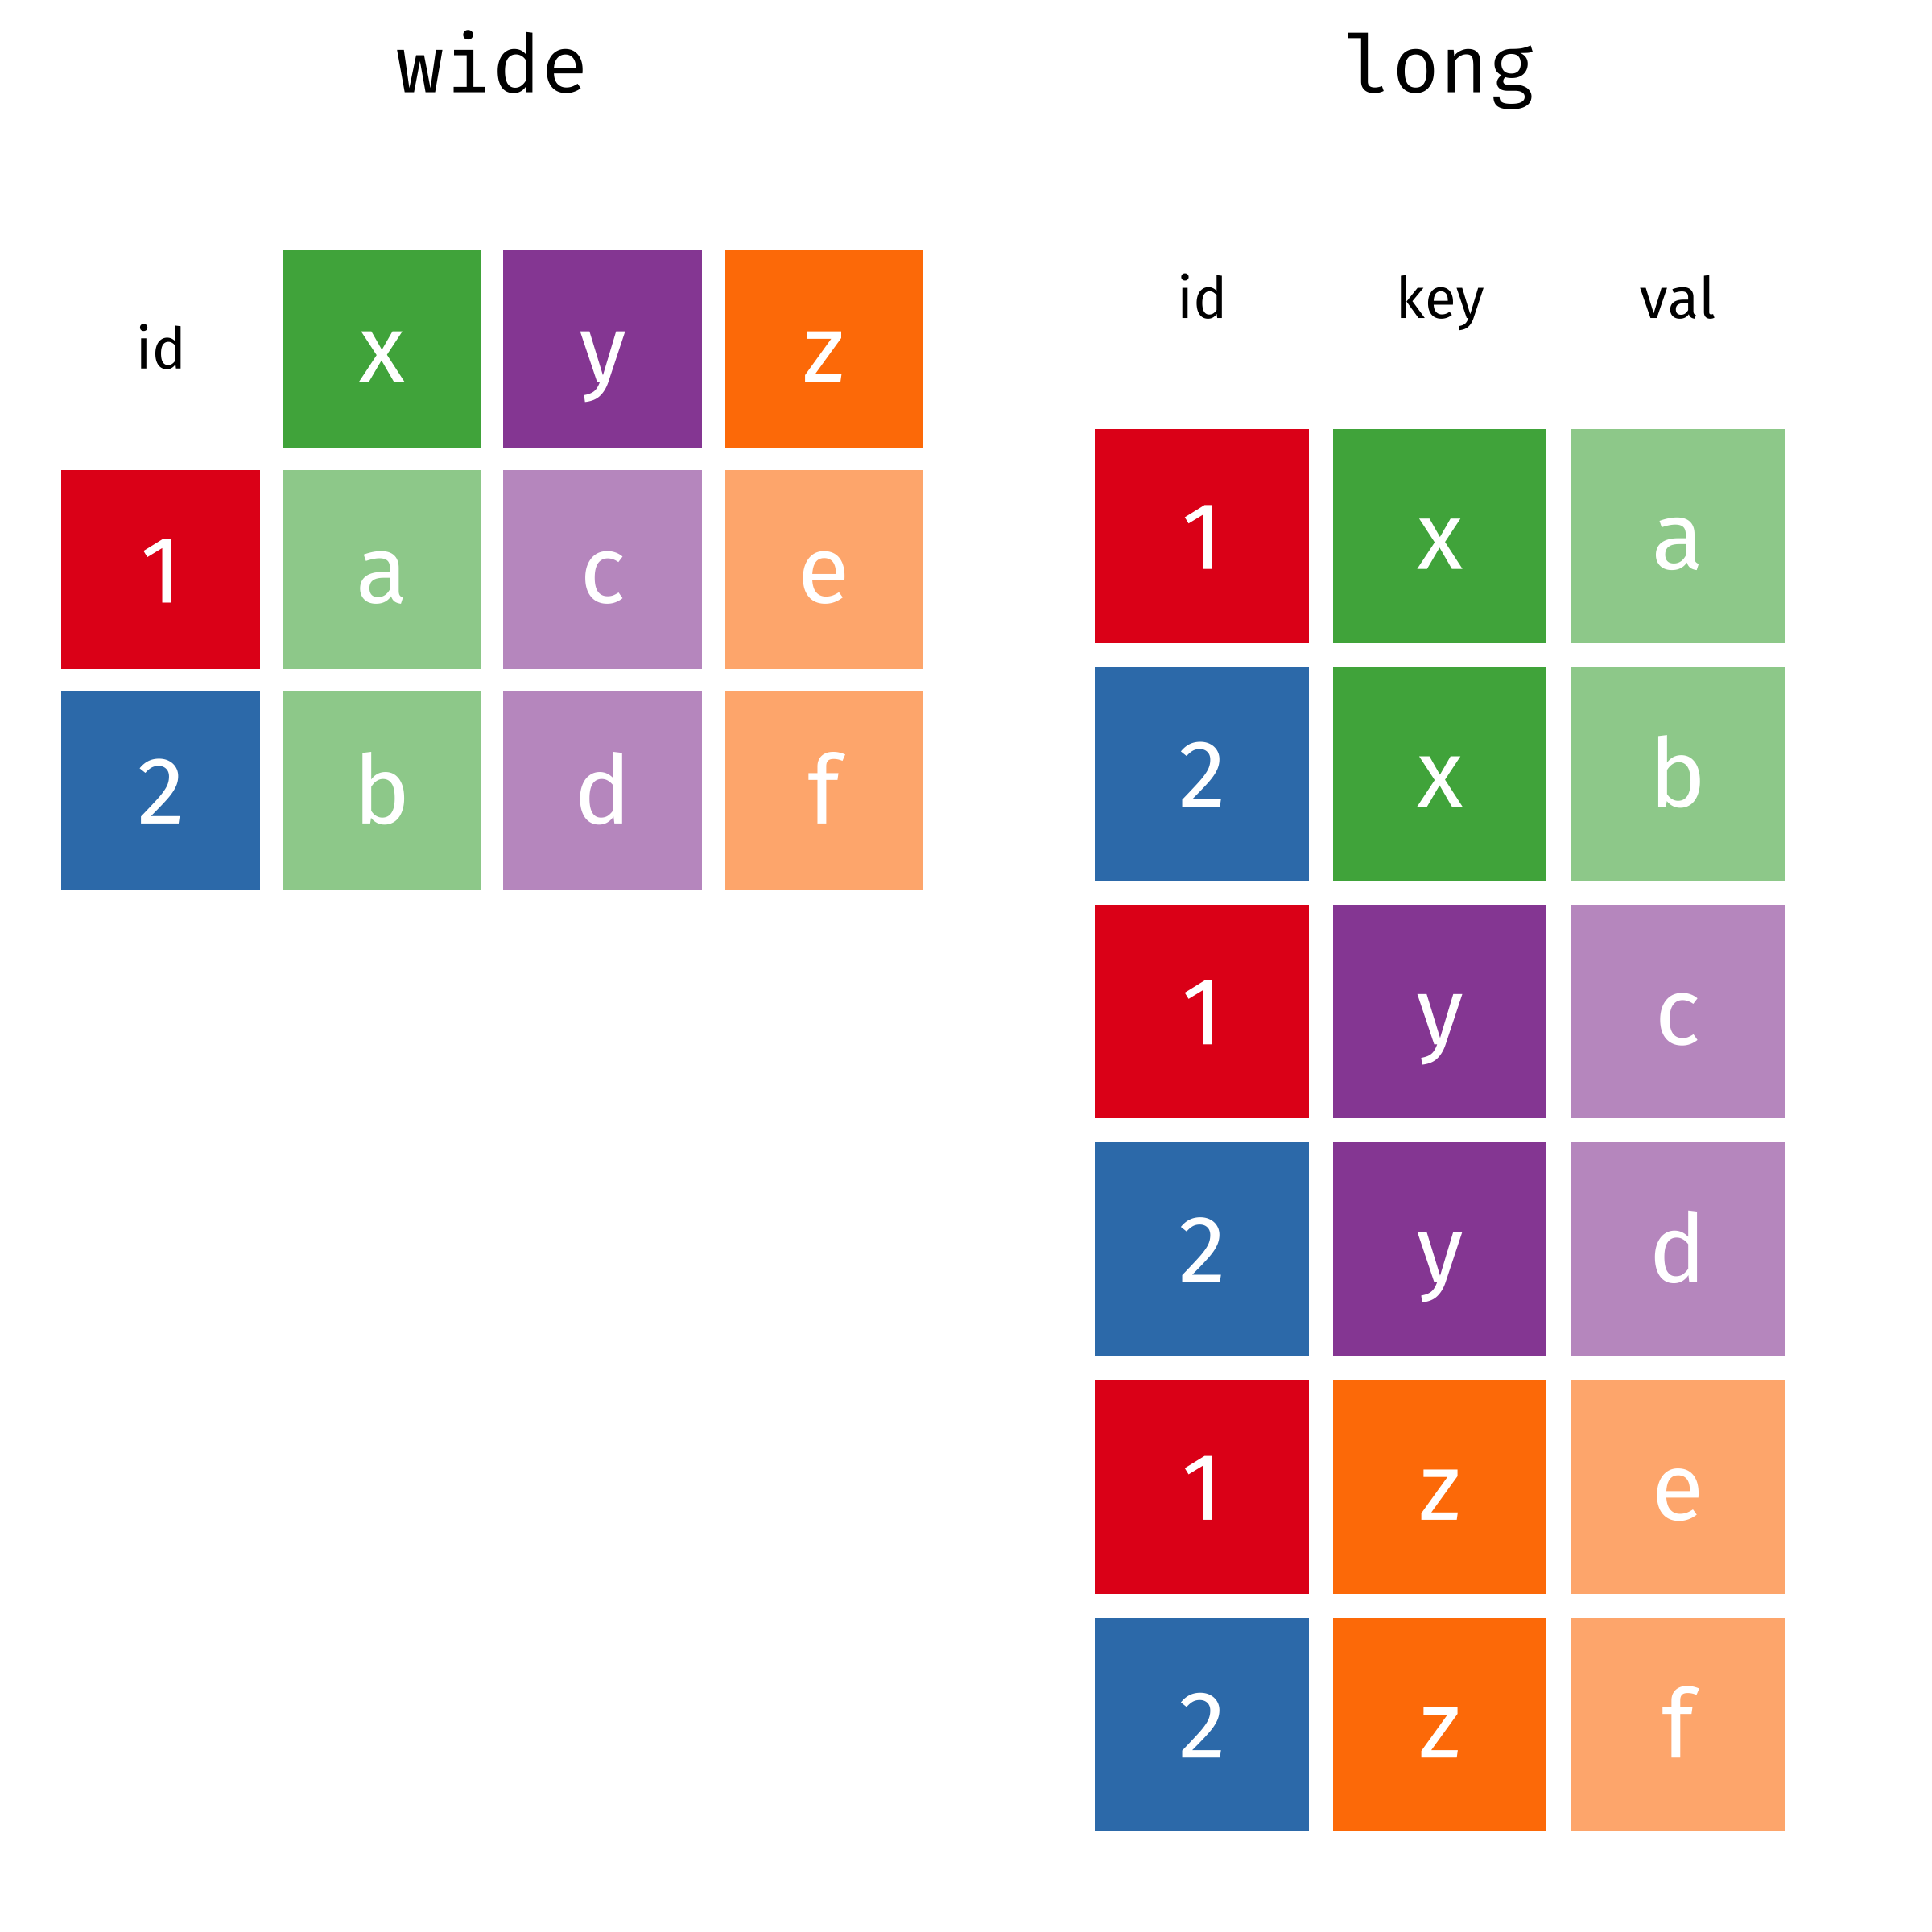
\includegraphics[width=0.5\textwidth,height=\textheight]{./img/long-wide-anim.png}

}

\caption{\label{fig-long-wide-anim}Links: Eine Tabelle mit Format
``wide'' - nicht ``tidy''. Rechts: Das ``Langformat'' ist tidy.}

\end{figure}

\begin{tcolorbox}[enhanced jigsaw, titlerule=0mm, bottomrule=.15mm, opacitybacktitle=0.6, colframe=quarto-callout-tip-color-frame, title=\textcolor{quarto-callout-tip-color}{\faLightbulb}\hspace{0.5em}{Tipp}, coltitle=black, colback=white, arc=.35mm, breakable, toptitle=1mm, opacityback=0, bottomtitle=1mm, left=2mm, leftrule=.75mm, rightrule=.15mm, toprule=.15mm, colbacktitle=quarto-callout-tip-color!10!white]

In fast allen Organisationen werden Exceltabellen zur Datenverarbeitung
verwendet. Dabei wiederholen sich immer wieder die gleichen Fehler bzw.
suboptimalen Vorgehensweise zum Aufbau einer Exceltabelle.

\href{https://www.tandfonline.com/doi/full/10.1080/00031305.2017.1375989}{Dieser
Artikel} von Broman und Woo (2018) zeigt anhand einiger praktischer
Tipps, wie man Exceltabellen so aufbaut, dass Fehler minimiert werden.

\end{tcolorbox}

\hypertarget{arten-von-variablen}{%
\subsection{Arten von Variablen}\label{arten-von-variablen}}

\hypertarget{nach-position-in-der-forschungsfrage}{%
\subsubsection{Nach Position in der
Forschungsfrage}\label{nach-position-in-der-forschungsfrage}}

Angenommen, Ihre Forschungsfrage lautet:

\begin{quote}
Hat Lernen einen Einfluss auf den Prüfungserfolg?
\end{quote}

In dem Fall gilt:

\begin{itemize}
\tightlist
\item
  \emph{Lernen} ist die Inputvariable/X-Variable/Ursache/UV
\item
  \emph{Prüfungserfolg} ist die Outputvariable/Y-Variable/Wirkung/AV
\end{itemize}

Abbildung~\ref{fig-ueberblick-fragen} stellt diese beiden ``Positionen''
einer Variable dar. Die erste Position ist vor dem Pfeil. Die zweite
Position ist nach dem Pfeil.

\begin{figure}

{\centering 

\begin{figure}[H]

{\centering 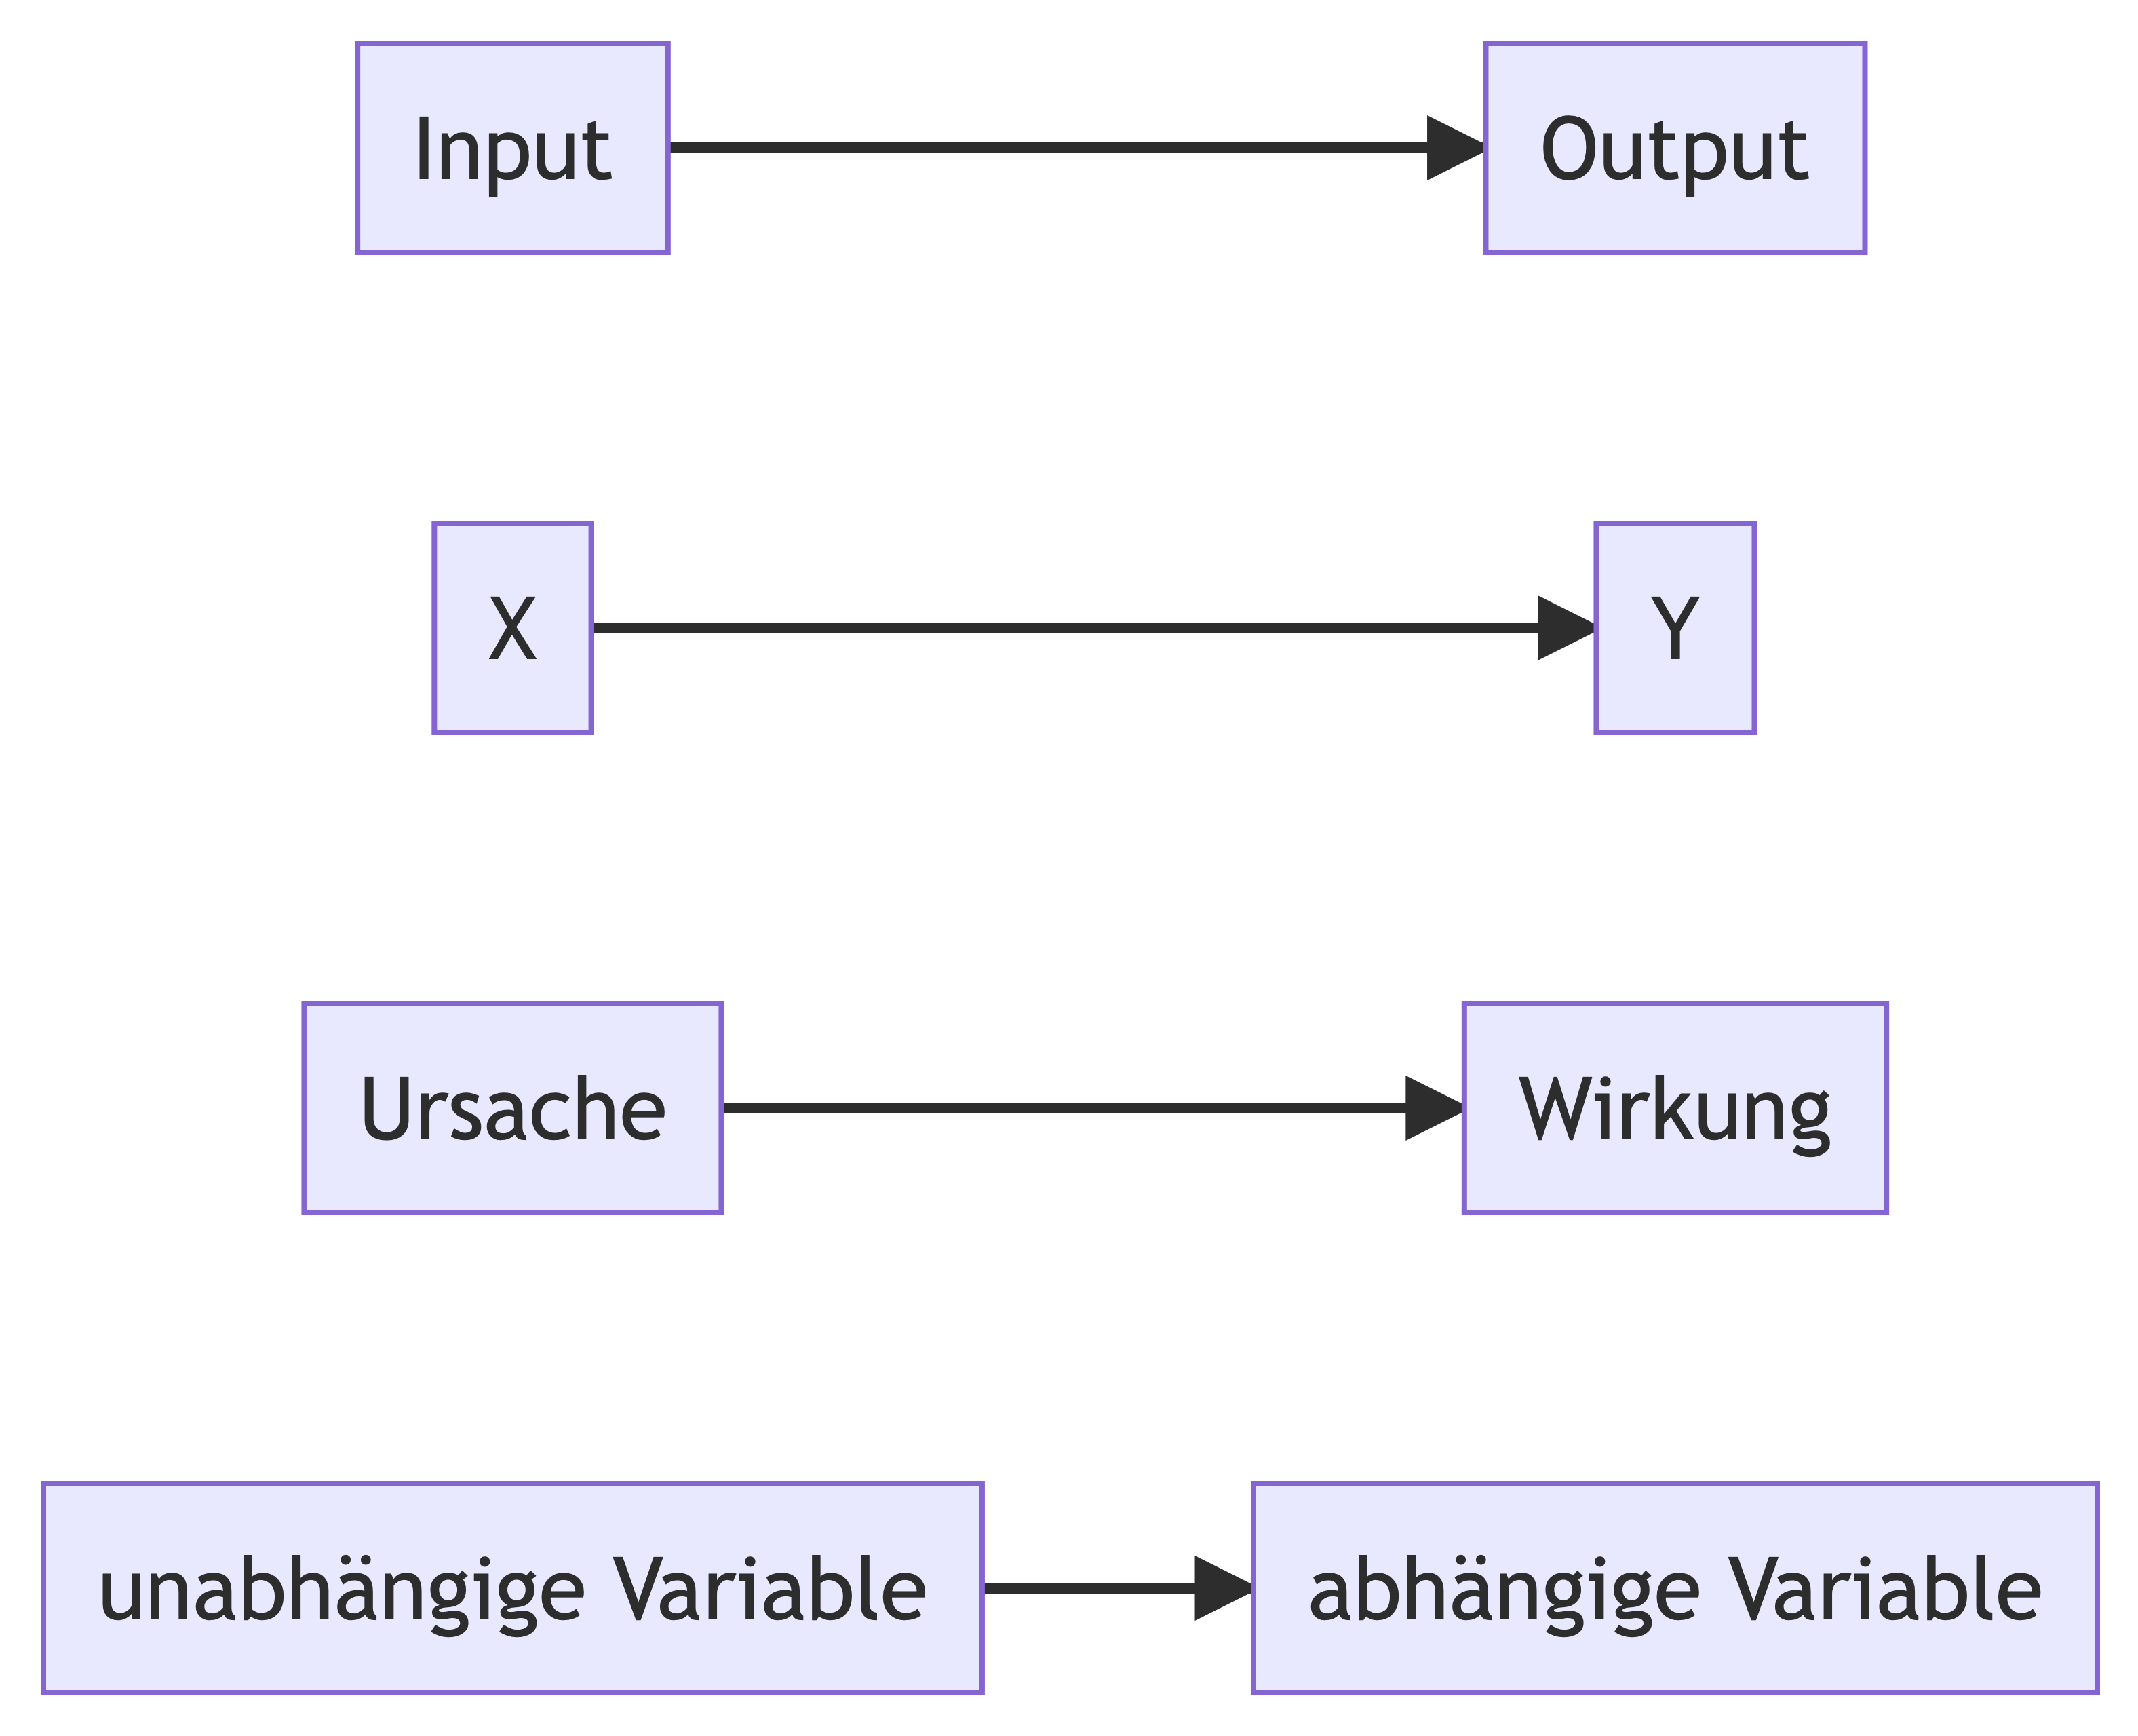
\includegraphics[width=4.11in,height=3.33in]{./fragenstellen_files/figure-latex/mermaid-figure-3.png}

}

\end{figure}

}

\caption{\label{fig-ueberblick-fragen}Überblick über den Inhalt und
Verlauf des Buches}

\end{figure}

\hypertarget{nach-dem-skalenniveau}{%
\subsubsection{Nach dem Skalenniveau}\label{nach-dem-skalenniveau}}

Abbildung~\ref{fig-skalenniveau} gibt einen Überblick über typisch
verwendete Skalenniveaus.

\begin{figure}

{\centering 

\begin{figure}[H]

{\centering 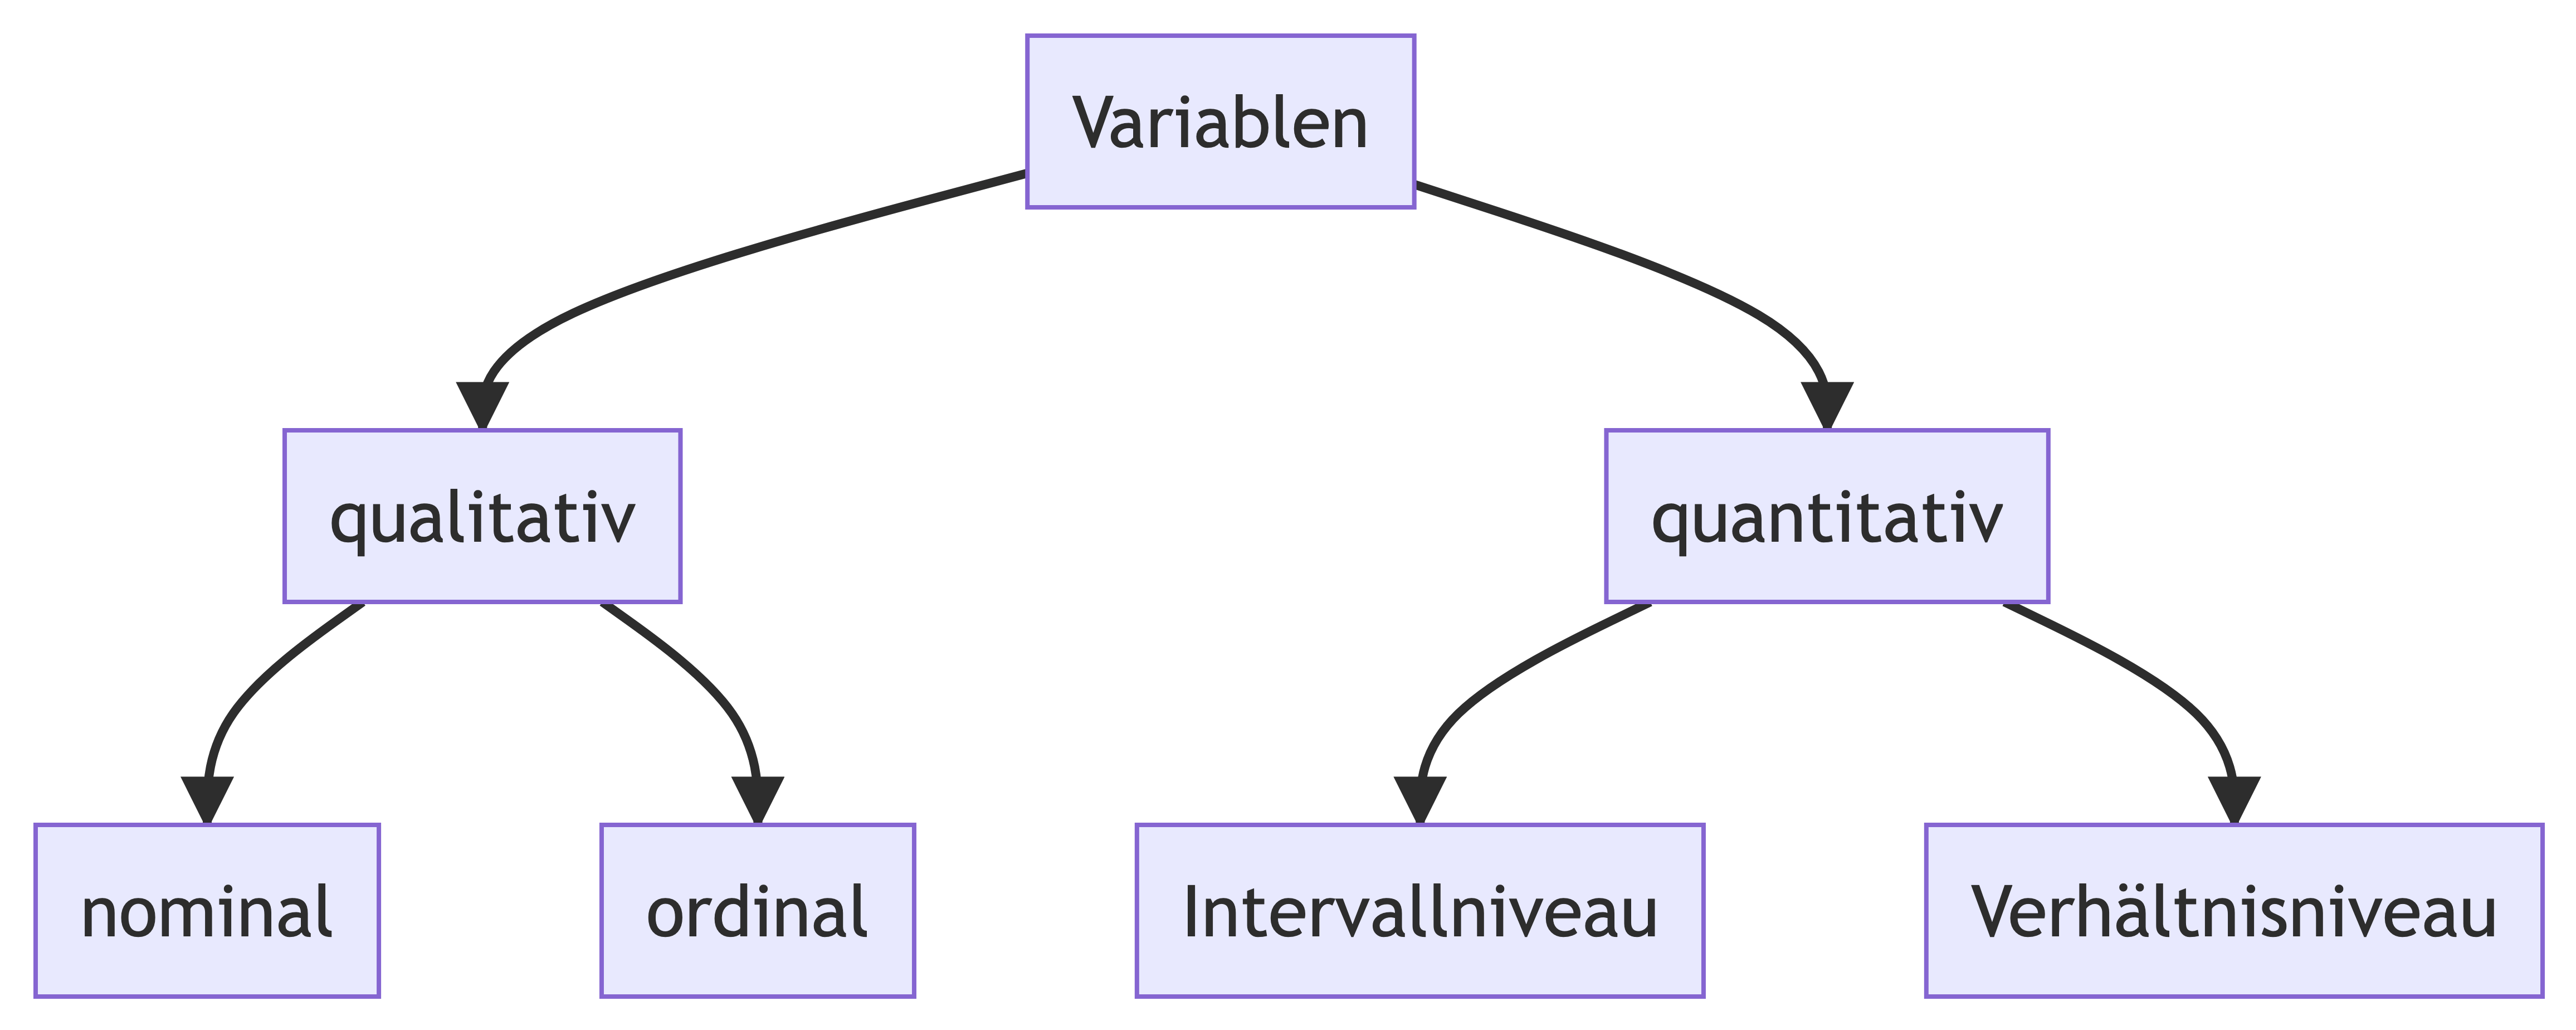
\includegraphics[width=6.03in,height=2.41in]{./fragenstellen_files/figure-latex/mermaid-figure-2.png}

}

\end{figure}

}

\caption{\label{fig-skalenniveau}Skalenniveaus}

\end{figure}

\hypertarget{beispiele-fuxfcr-skalenniveaus}{%
\section{Beispiele für
Skalenniveaus}\label{beispiele-fuxfcr-skalenniveaus}}

Beispiele zu den Skalenniveaus sind in Tabelle~\ref{tbl-skalen-bsps}
aufgeführt.

\hypertarget{tbl-skalen-bsps}{}
\begin{longtable}[]{@{}ll@{}}
\caption{\label{tbl-skalen-bsps}Beispiele für
Skalenniveaus}\tabularnewline
\toprule()
Variable & Skalenniveau \\
\midrule()
\endfirsthead
\toprule()
Variable & Skalenniveau \\
\midrule()
\endhead
Haarfarbe & Nominalskala \\
Augenfarbe & Nominalskala \\
Geschlecht & Nominalskala \\
Automarke & Nominalskala \\
Partei & Nominalskala \\
Lieblingsessen & Ordinalskala \\
Medaillen beim 100-Meter-Lauf & Ordinalskala \\
Uniranking & Ordinalskala \\
IQ & Intervallskala \\
Extraversion & Intervallskala \\
Temperatur in Celcius & Intervallskala \\
Temperatur in Fahrenheit & Intervallskala \\
Temperatur in Kelvin & Verhältnisskala \\
Körpergröße & Verhältnisskala \\
Geschwindigkeit & Verhältnisskala \\
Länge & Verhältnisskala \\
\bottomrule()
\end{longtable}

Je nach dem, über welches Skalenniveau eine Variable verfügt, sind
verschiedenen Rechenoperationen erlaubt, s.
Tabelle~\ref{tbl-skalenniveaus}.

\hypertarget{tbl-skalenniveaus}{}
\begin{longtable}[]{@{}llllll@{}}
\caption{\label{tbl-skalenniveaus}Erlaubte Rechenoperationen nach
Skalenniveau}\tabularnewline
\toprule()
Skalenniveau & Quantitativ & ≠ & ≼ & + & × \\
\midrule()
\endfirsthead
\toprule()
Skalenniveau & Quantitativ & ≠ & ≼ & + & × \\
\midrule()
\endhead
Nominalniveau & nein & ✅ & ❌ & ❌ & ❌ \\
Ordinalniveau & nein & ✅ & ✅ & ❌ & ❌ \\
Intervallniveau & ja & ✅ & ✅ & ✅ & ❌ \\
Verhältnisniveau & ja & ✅ & ✅ & ✅ & ✅ \\
\bottomrule()
\end{longtable}

Was soll das bedeuten, ``Rechenoperationen''?

Schauen wir uns für jedes Skalenniveau ein ``Rechenbeispiel'' an.

\emph{Nominalskala}: Die Variable \emph{Geschlecht} ist nominalskaliert.
Das bedeutet, dass ihre Ausprägungen \emph{Frau} und \emph{Mann} z.B.
nicht (sinnvoll) addiert oder sonswie ``verrechnet'' werden können. Man
könnte, z.B. um das Eintippen zu erleichtern, Frauen mit \texttt{1}
kodieren und Männer mit \texttt{2}. Damit darf man aber nicht rechnen!
Es macht keinen Sinn zu sagen: ``Ich habe eine Frau und einen Mann in
meiner Tabelle, das ist im Schnitt ein diverses Geschlecht, weil der
Mittelwert von 1 und 2 ist 1,5!''

Die \emph{einzige} ``Rechenoperation'', die man auf der Nominalskala
machen darf, ist die Prüfung auf Gleichheit: Mann kann feststellen, ob
ein Objekt gleich zu einem anderen ist oder unterschiedlich. Also ob
zwei Personen das gleiche Geschlecht haben oder von unterschiedlichem
Geschlecht sind. Etwas formaler ausgedrückt:

\begin{itemize}
\tightlist
\item
  👩 \(\ne\) 👨
\item
  👩 \(=\) 👩
\item
  👨 \(=\) 👨
\end{itemize}

\emph{Ordinalskala}: Diese Skala entspricht einer Rangordnung. Eine
Rangordnung ist etwa die geordnete Abfolge Ihres
Leibgerichte\footnote{1. Pizza, 2. Spagetthi, 3. Schnitzel}. Etwas
formaler ausgedrückt:

\begin{itemize}
\tightlist
\item
  🍕 \(\succ\) 🍝 \(\succ\) 🥩
\end{itemize}

Das komische Zeichen \(\succ\) soll heißen: ``Ist auf meiner Liste von
Leibgerichten weiter oben, mag ich lieber''. Man kann aber \emph{nicht}
sagen, ``Ich mag aber Pizza um 42\% mehr als die Spagetthi und die
wieder um 73\% mehr als ein Schnitzel!''. Zumindest kann man das nicht
ohne weitere Informationen und Annahmen. Es gibt also Dinge auf der
Welt, die man leicht in eine Rangordnung bringen kann, aber die man nur
schwer in der Größe der Unterschiede bemessen kann. Das ist die
Ordinalskala, s. Abbildung~\ref{fig-ordinal}.

\begin{figure}

{\centering 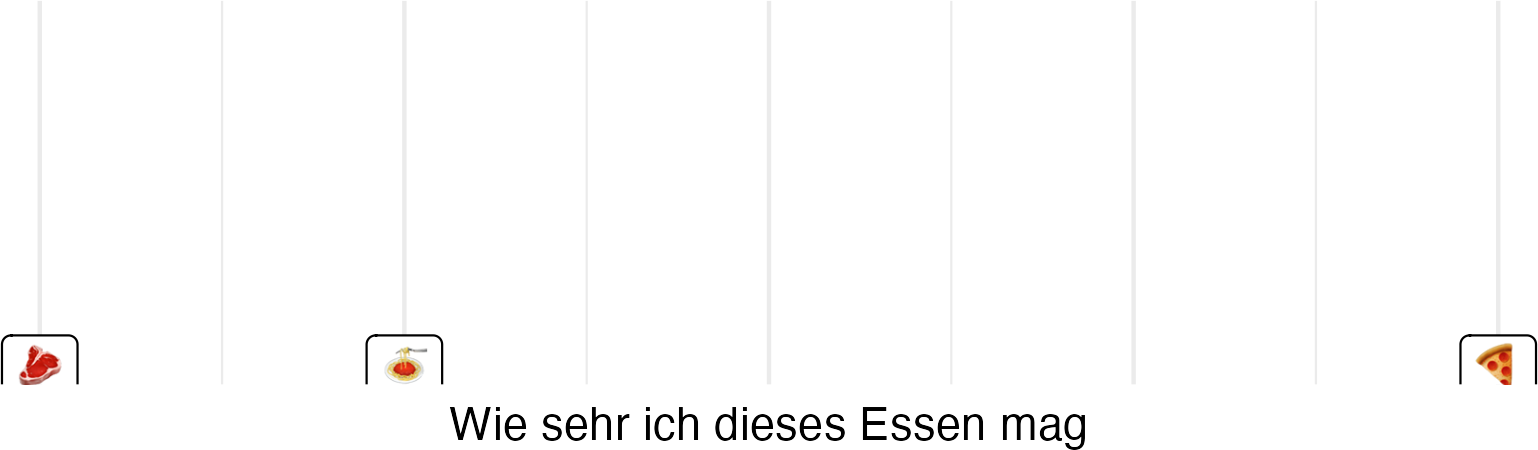
\includegraphics[width=1\textwidth,height=\textheight]{./fragenstellen_files/figure-pdf/fig-ordinal-1.png}

}

\caption{\label{fig-ordinal}Die Ordinalskala: Je weiter rechts auf der
X-Achse, desto höher lieber esse ich das Gericht.}

\end{figure}

\emph{Intervallskala}: Das ist vielleicht eine Überraschung für Sie:
Wenn es heute 10°C hat und morgen 5°C -- dann ist es heute \emph{nicht}
doppelt so warm wie morgen. Ja, 10 ist das Doppelte von 5. Aber
\emph{10° Celcius} ist nicht doppelt so warm wie 20° Celcius. Wenn Sie
das verwundert: Das ist normal, so geht es den meisten, wenn sie das zum
ersten Mal hören. Der Grund, dass es nicht erlaubt ist, Verhältnisse
(wie doppelt/halb so viel etc.) auf der Celcius-Skala zu bilden, ist,
dass der Nullpunkt der Skala, 0° C, kein echter, physikalischer
Nullpunkt ist. Bei 0° C liegt eben nicht Null Wärmeenergie vor.
Stattdessen wurde eine Wärmenergiemenge gewählt, die für uns Menschen
ganz praktisch, da augenfällig ist: der Gefrierpunkt von Wasser. Was bei
der Intervallskala erlaubt ist, ist das Addieren (und Subtrahieren):
heute 10°C, morgen 5°C, das ist ein Unterschied von 5°C. Oder: Im
Schnitt waren es 7,5°C, das ist genau in der Mitte von 5 und 10°C.
Abbildung~\ref{fig-intervall} versinnbildlicht die Intervallskala.

\begin{figure}

{\centering 
\includegraphics[width=1\textwidth,height=\textheight]{./fragenstellen_files/figure-pdf/fig-intervall-1.png}

}

\caption{\label{fig-intervall}Ein Metermaß steckt im Wasser. Auf dem
Metermaß können wir die aufgedruckten Zahlen ablesen. Aber wir wissen
nicht, ob der Metermaß auf dem Boden steht. Wir wissen demnach nicht, ob
der vom Metermaß angegebene Nullpunkt der wahre Nullpunkt (Meeresboden)
ist.}

\end{figure}

\emph{Verhältnisskala}: Eine Verhältnisskala ist das, was man sich
gemeinhin unter einer metrische Variable vorstellt: Man kann ``normal''
rechnen, alle Rechenoperationen sind erlaubt. Zuzüglich zu denen, die
auch in anderen, ``niedrigeren'' Skalenniveaus erlaubt sind, ist das das
Bilden von Verhältnissen - Multiplizieren, s.
Abbildung~\ref{fig-verhaeltnis}.

\begin{figure}

{\centering 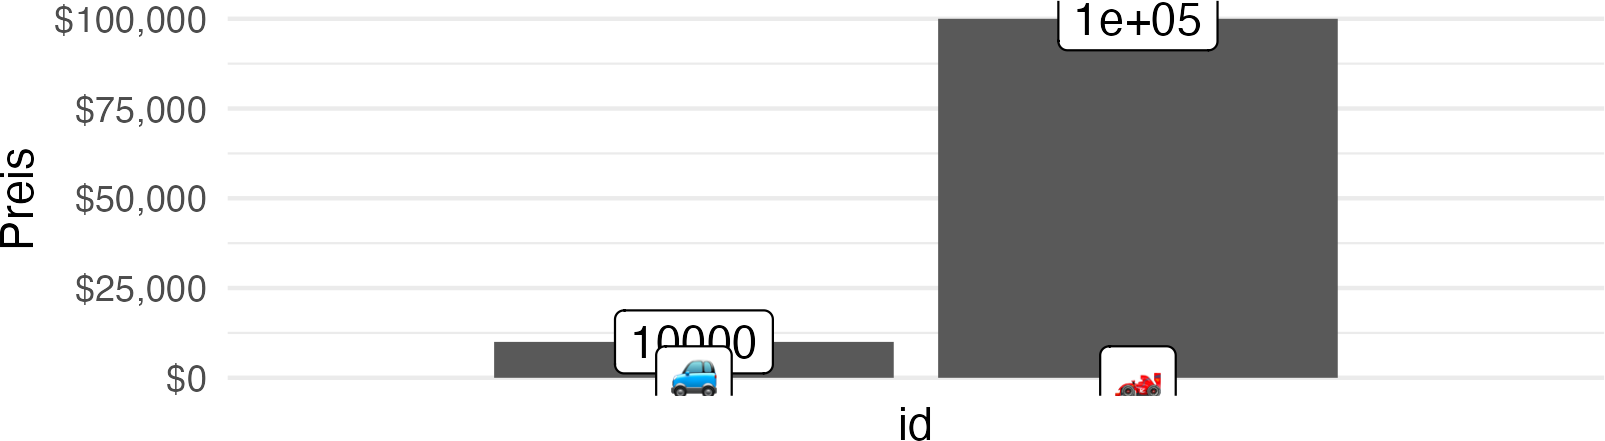
\includegraphics{./fragenstellen_files/figure-pdf/fig-verhaeltnis-1.png}

}

\caption{\label{fig-verhaeltnis}Puh! Der rote Flitzer ist 10 Mal so
teuer wie die blaue Möhre. Kohlen zusammenkratzen.''}

\end{figure}

In \href{https://www.youtube.com/watch?v=_mN3kFe56ng}{diesem Video} gibt
es noch ausführlichere Erklärung zum Thema Skalenniveaus.

\url{https://www.youtube.com/embed/wo9vZccmqwc}

Außerdem können quantitative Variablen untergliedert werden in:

\begin{itemize}
\tightlist
\item
  \emph{stetige} Variablen, das sind Variablen, bei denen man zwischen
  zwei Ausprägungen immer noch eine weitere quetschen kann. So gibt es
  eine Wert für die Köpergröße zwischen 1.60m und 1.61. Und einen Wert
  zwischen 1.601m und 1.602m, etc.
\item
  diskrete Variablen, das sind metrische Variablen, die nur bestimmte
  Ausprägungen haben, häufig sind das die natürlichen Zahlen:
  \(1,2,...\). Ein Beispiel wäre die Anzahl der Kinder in einer Familie.
\end{itemize}

\begin{tcolorbox}[enhanced jigsaw, titlerule=0mm, bottomrule=.15mm, opacitybacktitle=0.6, colframe=quarto-callout-tip-color-frame, title=\textcolor{quarto-callout-tip-color}{\faLightbulb}\hspace{0.5em}{Tipp}, coltitle=black, colback=white, arc=.35mm, breakable, toptitle=1mm, opacityback=0, bottomtitle=1mm, left=2mm, leftrule=.75mm, rightrule=.15mm, toprule=.15mm, colbacktitle=quarto-callout-tip-color!10!white]

Fragen nach Skalenniveaus gehören zu den Lieblingsprüfungsfragen in
diesem Themenbereich. Sie sind gut beraten, sich gerade mit dieser Frage
intensiver zu beschäftigen. Auch in thematisch angrenzenden Fächern wird
immer wieder die Frage nach dem Skalennvieau aufgeworfen. Das zeigt
natürlich auch die hohe Relevanz des Themas.

\end{tcolorbox}

\hypertarget{modelle}{%
\section{Modelle}\label{modelle}}

Woran denken Sie beim Wort ``Modell''? Vielleicht an Spielzeugautos, s.
Abbildung~\ref{fig-matchbox}.

\begin{figure}

{\centering 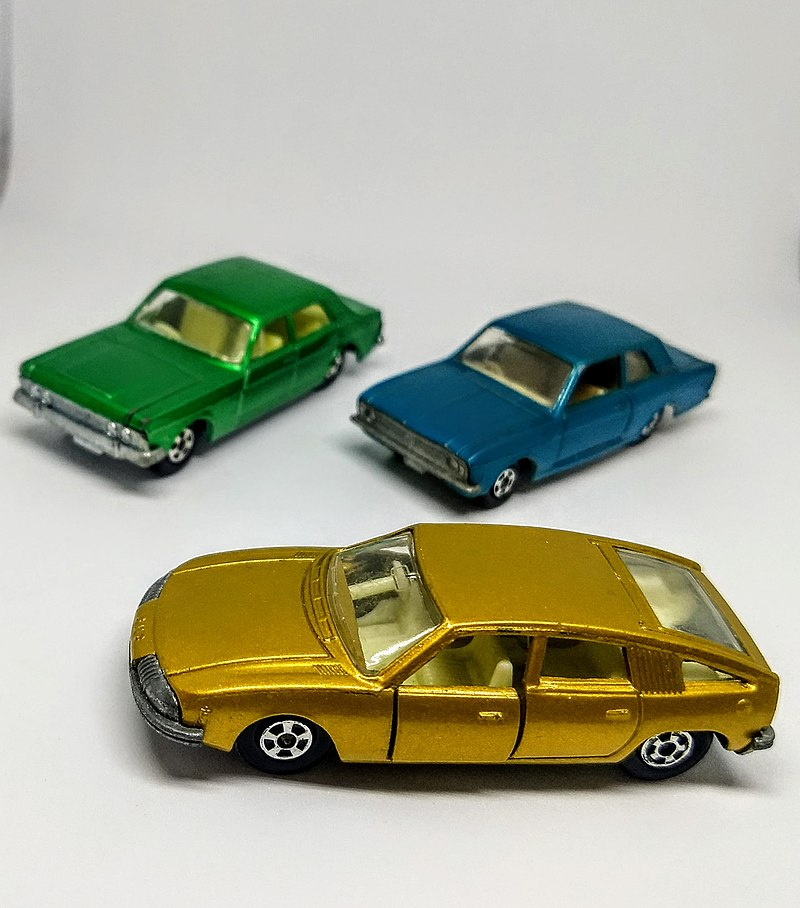
\includegraphics[width=0.25\textwidth,height=\textheight]{./img/matchbox.jpg}

}

\caption{\label{fig-matchbox}Matchbox-Autos sind Modelle für Autos}

\end{figure}

\leavevmode\vadjust pre{\hypertarget{def-modelle}{}}%
\begin{definition}[Modelle]\label{def-modelle}

Modelle sind ein vereinfachtes Abbild der Realität eine
\emph{Repräsentation} (Kaplan 2009).

\end{definition}

\leavevmode\vadjust pre{\hypertarget{exm-Modelle}{}}%
\begin{example}[Beispiele für Modelle]\label{exm-Modelle}

Puppen sind Modelle für Babies, Landkarten für Landstriche und
\href{https://de.wikipedia.org/wiki/Bohrsches_Atommodell}{das Atommodell
von Nils Bohr} ist ein Modell für Atome.

\end{example}

Auch in der Statistik nutzen wir Modelle. Helfen Sie Prof.~Weiss-Ois: Er
blickt nicht durch. Gerne würde er wissen, wie viele Stunden seine
Studentis auf die Prüfung lernen. Aber mit so vielen Zahlen kann er
nicht umgehen \ldots{} Geben Sie ihm ein Modell: Sagen Sie ihm, wie lang
die Studis typischerweise lernen (sagen Sie ihm ein einfach den
Mittelwert der Lernzeiten).

12, 8, 10, 11, 10, 9, 13, 9, 14, 9, 12, 14, 7, 9, 9, 11, 9, 4, 5, 12, 9,
6, 9, 12, 13, 9, 9, 6, 10, 8

\begin{figure}

{\centering 
\includegraphics[width=0.25\textwidth,height=\textheight]{./img/teacher.png}

}

\caption{Oh jeh, so viele Zahlen! Ich check nix! Wie viel lernen denn
jetzt meine Studis?!}

\end{figure}

\textbf{9.6}

\begin{figure}

{\centering 
\includegraphics[width=0.25\textwidth,height=\textheight]{./img/teacher.png}

}

\caption{Yeah, jetzt weiß ich, wie viel die Studis so typischerweise
lernen. Viel zu wenig natürlich!}

\end{figure}

\href{https://www.flaticon.com/free-icons/professor}{Icon unter Flaticon
licence, Autor: iconixar}

Der Nutzen von Modellen ist, dass sie komplexe Sachverhalte vereinfachen
und damit oft überhaupt erst einer Untersuchung zugänglich. In der
Datenanalyse bzw. Statistik\footnote{die beiden Begriffe werden hier
  weitgehend synonym gebraucht} fassen Sie oft viele Daten prägnant
zusammen, z.B. zu einer einzelnen Kennzahl.

\hypertarget{praxisbezug}{%
\section{Praxisbezug}\label{praxisbezug}}

Wir leben im Datenzeitalter; Daten durchdringen alle Bereiche des
beruflichen, gesellschaftlichen und privaten Lebens. Die Datenanalyse
hat sich in den letzten Jahren massiv verändert, s.
Abbildung~\ref{fig-fo-früher-heute}.

\begin{figure}

{\centering 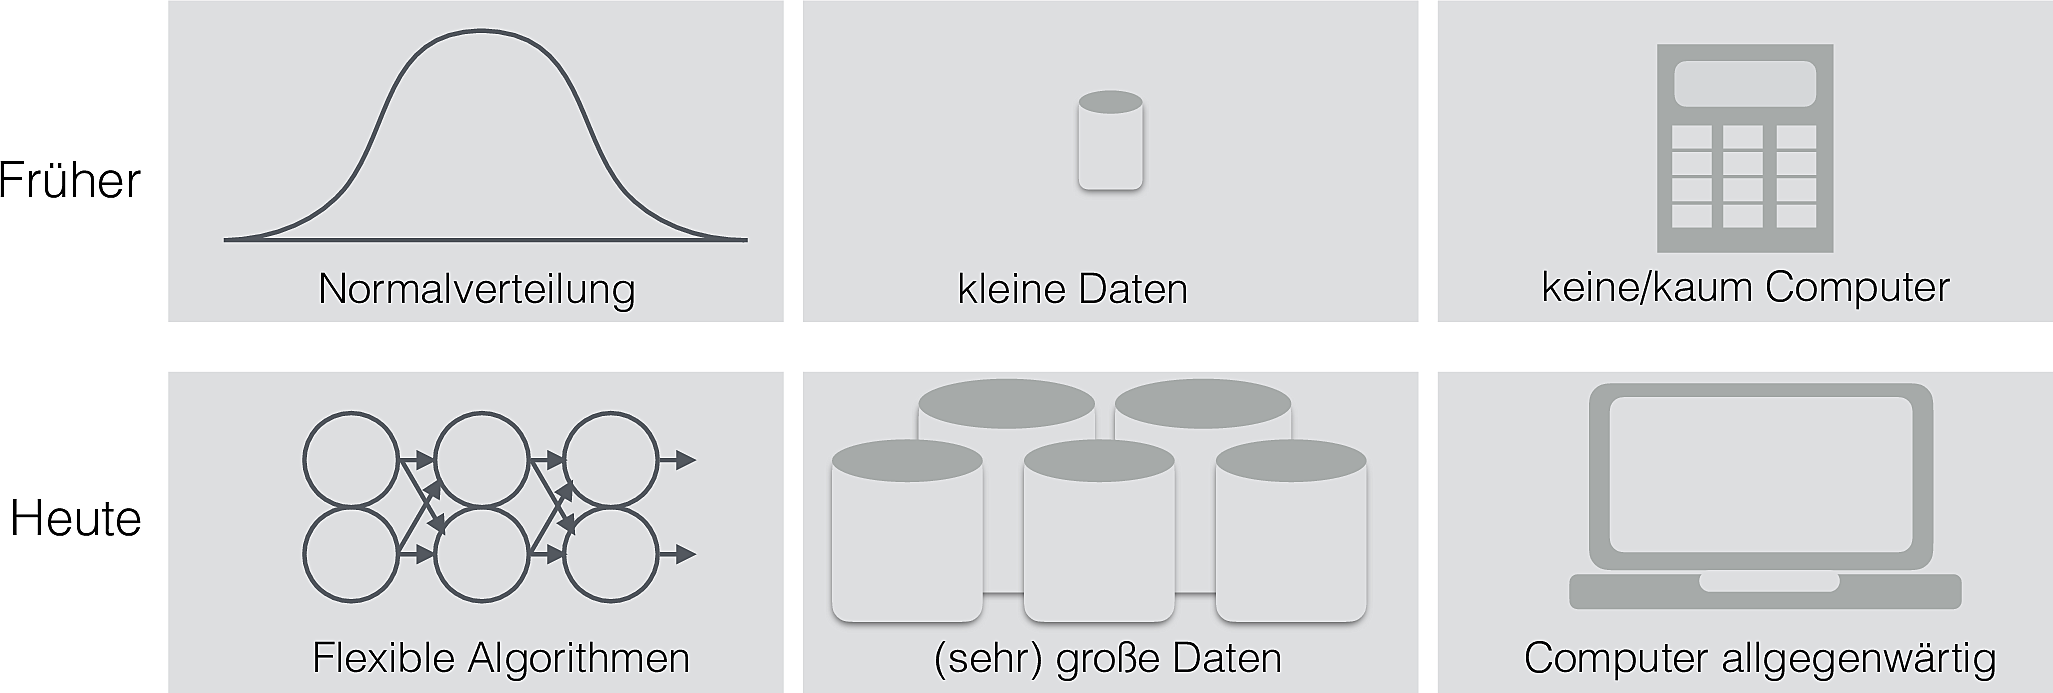
\includegraphics{./img/Forschung_frueher_heute-crop.png}

}

\caption{\label{fig-fo-früher-heute}Forschung früher und heute}

\end{figure}

Diese Entwicklung ist durchaus auch kritisch zu betrachten. Mit der
wachsenden Bedeutung von Daten wächst in gleichem Maße die Bedeutung von
Datenanalyse. Denn Daten ohne Sinn sind nutzlos. Aus diesem Grund kann
man sagen, dass Datenanalyse (und damit auch Statistik als eine
spezielle Art von Datenanalyse) zu stark nachgefragten Jobs gehören.

Laut \href{https://web.arbeitsagentur.de/entgeltatlas/beruf/129987}{dem
Entgeltatlas der Bundesagentur für Arbeit} liegt ein typisches Gehalt
von Data Scientisten bei knapp 6000 € pro Monat (in der Altersgruppe von
25 bis 54)\footnote{Abrufdatum: 1.2.23}. Laut dem
\href{https://gehaltsreporter.de/gehaelter-von-a-bis-z/it/data-scientist/}{Gehaltsreporter}
liegt das Einstiegsgehalt dieser Berufsgruppe bei knapp 50.000€ pro
Jahr.

\hypertarget{fazit}{%
\section{Fazit}\label{fazit}}

Die Aufgabe von Statistik ist es, durch Zusammenfassen von Daten Modelle
zu bilden, die es uns einfacher machen, schwierige Sachverhalte zu
verstehen. Zentral ist dabei, die Analyse von Variabilität der Daten.
Daten kommen in verschiedenen Varianten vor, typischerweise in
Tabellenform, möglichst im Tidy-Format.

\hypertarget{aufgaben}{%
\section{Aufgaben}\label{aufgaben}}

\begin{enumerate}
\def\labelenumi{\arabic{enumi}.}
\tightlist
\item
  \href{https://datenwerk.netlify.app/posts/variation01/variation01.html}{variation01}
\item
  \href{https://datenwerk.netlify.app/posts/def-statistik01/def-statistik01}{Def-Statistik01}
\item
  \href{https://datenwerk.netlify.app/posts/tidy1/tidy1.html}{tidy1}
\item
  \href{https://datenwerk.netlify.app/posts/skalenniveau1a/skalenniveau1a}{Skalenniveau1a}
\item
  \href{https://datenwerk.netlify.app/posts/ziele-statistik/ziele-statistik}{Ziele-Statistik}
\item
  \href{https://datenwerk.netlify.app/posts/variation02/variation02.html}{variation02}
\item
  \href{https://datenwerk.netlify.app/posts/skalenniveau1b/skalenniveau1b}{Skalenniveau1b}
\end{enumerate}

\hypertarget{vertiefung}{%
\section{Vertiefung}\label{vertiefung}}

\emph{nicht prüfungsrelevant}

\begin{enumerate}
\def\labelenumi{\arabic{enumi}.}
\tightlist
\item
  Fassen Sie den Artikel von Broman und Woo (2018) zusammen.
\end{enumerate}

\hypertarget{literatur-1}{%
\section*{Literatur}\label{literatur-1}}
\addcontentsline{toc}{section}{Literatur}

\hypertarget{refs}{}
\begin{CSLReferences}{1}{0}
\leavevmode\vadjust pre{\hypertarget{ref-broman_data_2018}{}}%
Broman, Karl W., und Kara H. Woo. 2018. {„Data Organization in
Spreadsheets``}. \emph{The American Statistician} 72 (1): 2--10.
\url{https://doi.org/10.1080/00031305.2017.1375989}.

\leavevmode\vadjust pre{\hypertarget{ref-kaplan_statistical_2009}{}}%
Kaplan, Daniel T. 2009. \emph{Statistical modeling: a fresh approach}.
Scotts Valley, Calif.: {CreateSpace}.
\url{https://dtkaplan.github.io/SM2-bookdown/}.

\leavevmode\vadjust pre{\hypertarget{ref-poldrack_statistical_2023}{}}%
Poldrack, Russell A. 2023. \emph{Statistical thinking: analyzing data in
an uncertain world}. Princeton: Princeton University Press.
\url{https://statsthinking21.github.io/statsthinking21-core-site/}.

\leavevmode\vadjust pre{\hypertarget{ref-schwaiger_impact_2022}{}}%
Schwaiger, Elizabeth, und Rameen Tahir. 2022. {„The impact of nomophobia
and smartphone presence on fluid intelligence and attention``}.
\emph{Cyberpsychology: Journal of Psychosocial Research on Cyberspace}
16 (1). \url{https://doi.org/10.5817/CP2022-1-5}.

\leavevmode\vadjust pre{\hypertarget{ref-ward_brain_2017}{}}%
Ward, Adrian F., Kristen Duke, Ayelet Gneezy, und Maarten W. Bos. 2017.
{„Brain Drain: The Mere Presence of One's Own Smartphone Reduces
Available Cognitive Capacity``}. \emph{Journal of the Association for
Consumer Research} 2 (2): 140--54. \url{https://doi.org/10.1086/691462}.

\leavevmode\vadjust pre{\hypertarget{ref-wickham_r_2018}{}}%
Wickham, Hadley, und Garrett Grolemund. 2018. \emph{R für Data Science:
Daten importieren, bereinigen, umformen, modellieren und visualisieren}.
Übersetzt von Frank Langenau. 1. Auflage. Heidelberg: O'Reilly.
\url{https://r4ds.had.co.nz/index.html}.

\leavevmode\vadjust pre{\hypertarget{ref-world_economic_forum_future_2020}{}}%
World Economic Forum. 2020. {„The Future of Jobs Report 2020``}.
{CH}-1223 Cologny/Geneva Switzerland: World Economic Forum.
\url{https://www3.weforum.org/docs/WEF_Future_of_Jobs_2020.pdf}.

\end{CSLReferences}



\end{document}
